\chapter{Results}\label{results}


\section{Data Acquisition}\label{data}

\begin{figure}
	\centering
	\begin{subfigure}{0.47\textwidth}
		\centering
		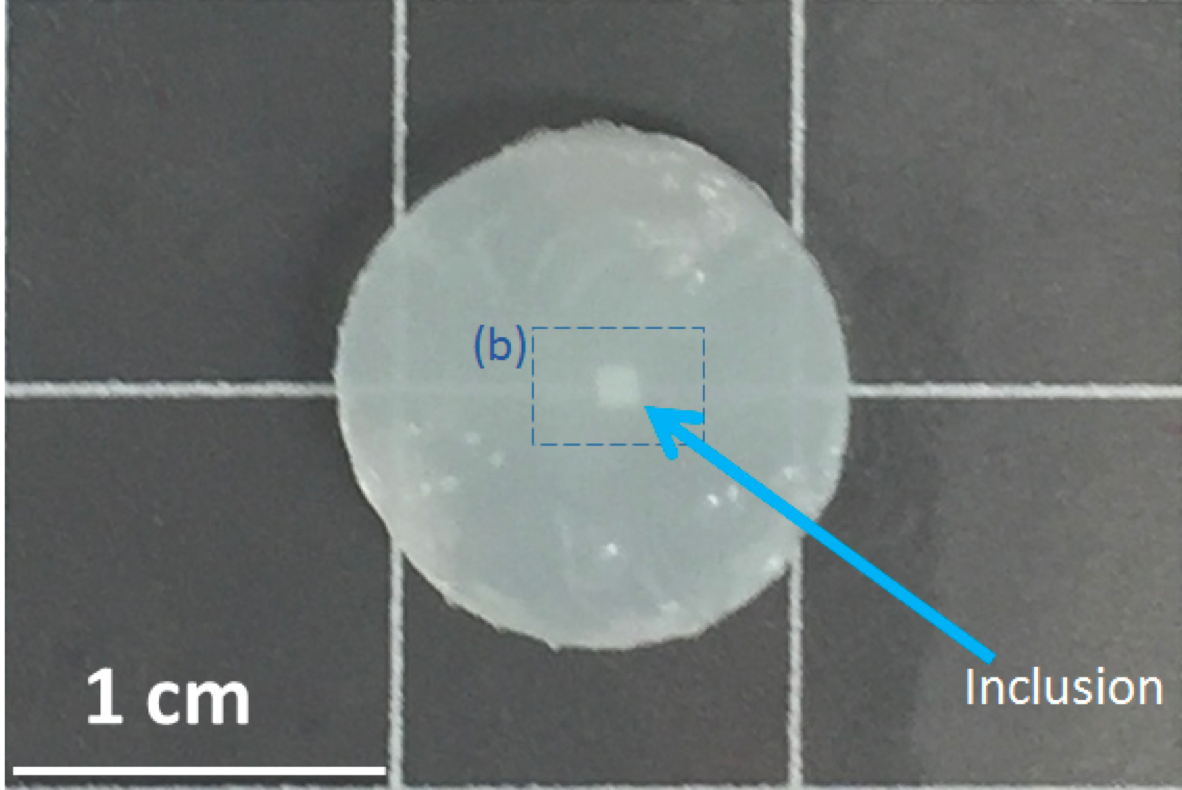
\includegraphics[width=\textwidth]{figures/phantom.png}
	\end{subfigure}
	\quad
	\begin{subfigure}{0.49\textwidth}
		\centering
		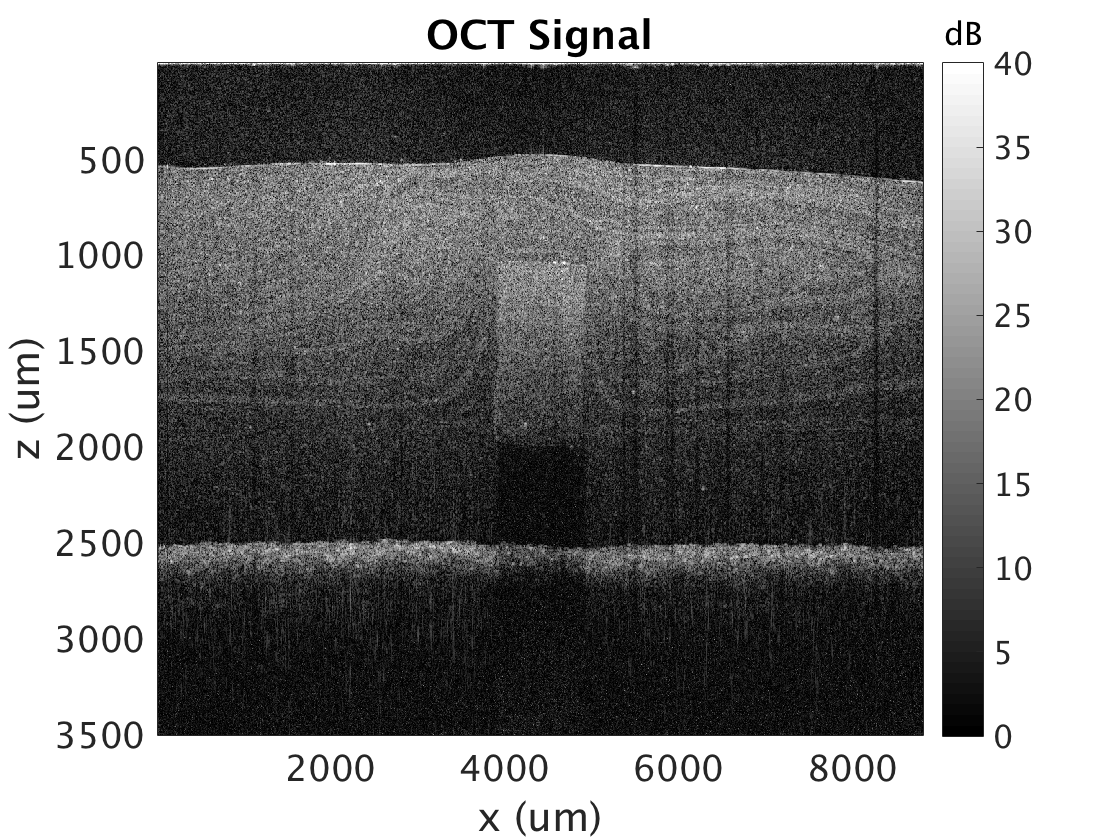
\includegraphics[width=\textwidth]{figures/oct.png}
	\end{subfigure}	
	\caption{The silicone phantom used to investigate strain estimation techniques a) photographed and b) imaged by the OCT system.}
	\label{oct_image}	
\end{figure}

To better quantify the image quality, an idealised silicone sample was imaged, to approximate breast tissue, and the strain estimated. This phantom consisted of a bulk, softer silicone material (with a Young's modulus of 6.4kPa) within which was a stiff, rectangular inclusion (Young's modulus of 100kPa) \cite{hepburn_improving_2017}, to which optical scatterers were added to enhance the OCT signal. The phantom was created by a previous Master's student, and was imaged using a desktop OCE system, with a system wavelength of $1300nm$. The imaged area, shown in \autoref{oct_image}, was divided into 2000 A-scans per each B-scan, over a length in x of $4.4\mu m$), and a total of 6817 B-scans were acquired, over the same length in y.

The complex OCT C-scan was initially processed from the raw spectral data produced by the Fourier-domain OCT system, to produce the complex OCT signal values, with associated optical amplitudes and random phase. From here, as described briefly in \autoref{compression_oce}, the difference in phase is calculated between loaded and unloaded B-scans, and averaged over 100 B-scans. The strain estimation algorithms described following utilise this calculated averaged phase difference as the beginning step of the processing pipeline, and assume that the phase difference data is already loaded into memory.

\section{Strain Estimation Algorithms}\label{algorithms}

A total of six different strain estimation algorithms were implemented and tested, and can be differentiated based on how the phase unwrapping issue is addressed, and the digital differentiation filter used. \autoref{flowchart} demonstrates the decision processes in these strain estimation algorithms that separate the way they get from the complex phase difference delivered by the OCT system and pre-processing, to the final strain elastogram image.

The functions worked by using the complex phase difference C-scan as an input, as well as the specifications for the fit (axial) and lateral resolutions of the system. The fit resolution of the system determined the fit window for the WLS and Savitzky-Golay based strain estimation techniques, and the axial Gaussian $\sigma$ value for the finite difference based techniques. The lateral resolution determined to what extent the strain images were laterally averaged by a Gaussian smoothing filter (for reasons discussed in the later section 4.3). If a lateral resolution of 0 was specified, no lateral smoothing was performed. 

\subsection{WLS with Unwrapped Phase}
The WLS with phase unwrapping algorithm unwraps the phase by reading in the entire volume and saves the unwrapped phase data to file. In a sequential loop over each B-scan, wrapped in a Matlab parfor parallel, the process reads in the complex phase and unwrapped phase for each B-scan. If lateral smoothing has been specified, it smooths the unwrapped phase using unweighted Gaussian smoothing by convoluting the unwrapped phase with the 1D lateral filter. A sequential looping is then performed over each A-scan and all fit segments within the given B-scan, which calculates the WLS estimate of strain using summations and the weights from the complex phase data.

\subsection{SG Filtering on Unwrapped Phase}
This function unwraps the phase by the same process specified above, which requires a read from file of the unwrapped phase for each B-scan. If lateral smoothing required, the unwrapped phase is similarly smoothed via convolution with an unweighted Gaussian smoothing filter. To estimate the strain, this smoothed unwrapped phase data is convolved with the analytically derived Savitzky-Golay filter in a single action of the entire B-scan.

\begin{figure}[th!]
\begin{tikzpicture}[node distance=2cm, remember picture]
	\centering
	\node [anchor=north] at (0,0) (input) [io] {INPUT: $\Delta\phi_i$};
    
    \node (volume_unwrap) at (-4,-3) [basic] {Unwrapping Algorithm};
    \draw [wls] (input.225) edge[out=270,in=90] (volume_unwrap.100);
    \draw [uwsg] (input.240) edge[out=270,in=90] (volume_unwrap.80);
    
    \node (bscan_loop) at (0,-5.5) [main_long] {LOOP OVER B-SCANS};
    \draw [wls] (volume_unwrap.260) edge[out=270,in=90] (bscan_loop.135);
    \draw [uwsg] (volume_unwrap.280) edge[out=270,in=90] (bscan_loop.120);
    \draw [posg] (input.260)--(bscan_loop.100);
    \draw [wfd] (input.280)--(bscan_loop.80);
    \draw [uwfd] (input.300)--(bscan_loop.60);
    \draw [fdsm] (input.315)--(bscan_loop.45);
    
   	\node (variance) at (-4,-8) [basic] {Calculate variances};
    \draw [wls] (bscan_loop.225) edge[out=270,in=90] (variance.90);
    
    \node (unweighted) at (4,-8) [basic] {Remove phase weighting};
    \draw [uwfd] (bscan_loop.300) edge[out=270,in=90] (unweighted.90); 
    
    \node (lateral) at (0,-10.5) [temp] {LATERAL SMOOTHING};
    \draw [uwsg] (bscan_loop.240)--(lateral.120);
    \draw [posg] (bscan_loop.260)--(lateral.100);
    \draw [wfd] (bscan_loop.280)--(lateral.80);
    \draw [fdsm] (bscan_loop.315)--(lateral.45);

    \draw [wls] (variance.270) edge[out=270,in=90] (lateral.135);
    \draw [uwfd] (unweighted.270) edge[out=270,in=90] (lateral.60);
    
    \node (fit_loop) at (-4,-13.5) [main] {LOOP OVER FIT SEGMENTS};
    \draw [wls] (lateral.225) edge[out=270,in=90] (fit_loop.100);
    \draw [posg] (lateral.260) edge[out=270,in=90] (fit_loop.80);
    
    \node (ascan_loop) at (-6.5,-16) [main] {LOOP OVER A-SCANS};
    \draw [wls] (fit_loop.260) edge[out=270,in=90] (ascan_loop.90);
    
    \node (wls_strain) at (-4,-18) [basic] {WLS strain estimation};
    \draw [wls] (ascan_loop.270) edge[out=270,in=90] (wls_strain.90);
    
    \node (phase_offset) at (-2.5,-16) [basic] {Divide complex phase offset};
    \draw [posg] (fit_loop.280) edge[out=270,in=90] (phase_offset.90);
    
    \node (sg_filter) at (0,-18) [basic] {Convolve with SG Filter};
    \draw [posg] (phase_offset.270) edge[out=270,in=90] (sg_filter.100);
    \draw [uwsg] (lateral.240) edge[out=270,in=90] (sg_filter.120);
   
   \node (gauss_filter) at (2,-15.8) [basic] {Convolve with an axial 1D Gaussian filter};
   \draw [wfd] (lateral.280) edge[out=270,in=90] (gauss_filter.100);
   \draw [uwfd] (lateral.300) edge[out=270,in=90] (gauss_filter.80);
   
   \node (pre_filter) at (6,-15.5) [basic] {Convolve with a small 2D Gaussian 'pre-filter'};
   \draw [fdsm] (lateral.315) edge[out=270,in=90] (pre_filter.90);
   
   \node (fd) at (4,-18) [basic] {FD strain estimation};
   \draw [wfd] (gauss_filter.260) edge[out=270,in=90] (fd.80);
   \draw [uwfd] (gauss_filter.280) edge[out=270,in=90] (fd.60);
   \draw [fdsm] (pre_filter.270) edge[out=270,in=90] (fd.45);
   
   \node (output) at (0,-20.5) [io] {OUTPUT: $\epsilon$};
   \draw [wls] (wls_strain.270) edge[out=270,in=90] (output.135);
   \draw [uwsg] (sg_filter.240) edge[out=270,in=90] (output.120);
   \draw [posg] (sg_filter.260) edge[out=270,in=90] (output.100);
   \draw [wfd] (fd.280) edge[out=270,in=90] (output.80);
   \draw [uwfd] (fd.300) edge[out=270,in=90] (output.60);
   \draw [fdsm] (fd.315) edge[out=270,in=90] (output.45);

    % LEGEND:
   \matrix[draw=black,rounded corners] at (6,-1) {  
    \node (m1) at (0.5,0) [empty] {};
    \node (wls) at (3,0) [legendtext] {UW WLS};
    \draw [wls] (m1)--(wls.west);
    \node (m2) at (0.5,-0.5) [empty] {};
    \node (uwsg) at (3,-0.5) [legendtext] {UW SG};
    \draw [uwsg] (m2)--(uwsg.west);
    \node (m3) at (0.5,-1) [empty] {};
    \node (posg) at (3,-1) [legendtext] {PO SG};
    \draw [posg] (m3)--(posg.west);
    \node (m4) at (0.5,-1.5) [empty] {};
    \node (wfd) at (3,-1.5) [legendtext] {WFD};
    \draw [wfd] (m4)--(wfd.west);
    \node (m5) at (0.5,-2) [empty] {};
    \node (uwfd) at (3,-2) [legendtext] {UWFD};
    \draw [uwfd] (m5)--(uwfd.west);
    \node (m6) at (0.5,-2.5) [empty] {};
    \node (fdsm) at (3,-2.5) [legendtext] {PF FD};
    \draw [fdsm] (m6)--(fdsm.west);
    \\
    };

\end{tikzpicture}
\caption{Flowchart of pivotal processes for the six different strain estimation techniques investigated: unwrapping with WLS (blue), unwrapping with SG filtering (orange), offset phase with SG filtering (yellow), weighted smoothing with FD (purple), unweighted smoothing with FD (green), and pre-filtered FD with weighted smoothing (light blue).}
\label{flowchart}
\end{figure}

\subsection{SG Filtering on Offset Phase}
In order to correct for phase unwrapping, the function reads in the complex phase for each B-scan (in a parallel Matlab parfor loop) and loops over all fit segments within the B-scan, taking a matrix of values across all A-scans for the given depths. Using Matlab's inbuilt bsxfun operator, an averaged complex phase value for each fit segment is calculated and divided (corresponding to subtraction of the phase) to move the phase values into an unwrapped region. The Savitzky-Golay filter, which was pre-calculated using the analytical solution, is then convolved with the matrix in the axial direction to produce the strain estimation values at that given depth. 

\subsection{FD on Weighted Smoothing of Phase Difference}
The complex weighted phase difference that acts as the function's input is smoothed using an axial Gaussian filter dependent on the fit resolution supplied (and a lateral filter if specified). For strain estimation, finite difference is performed using bsxfun on the complex phase data (in order to prevent the introduction of  wrapping artefacts), by dividing one pixel by the conjugate of the previous pixel in order to subtract the phase values. This estimate of the spatial derivative of the phase difference is then converted into strain values.

\subsection{FD on Unweighted Smoothing of Phase Difference}
This algorithm works almost identically to the one described in the previous section, except that prior to using a Gaussian smoothing filter on the complex phase data, the amplitude is normalised to 1 for all phase difference values, effectively removing the optical weighting that comes from the OCT signal. From here the finite difference is calculated, and from this the strain. 

\subsection{Pre-Filtered Phase Difference with Smoothed FD Strain}
The 'Pre-Filtered' phase difference algorithm was implemented as an effort to remove 'ripples' introduced by high intensity pixels in the finite difference with weighted smoothing described in Section 4.2.4, which will be discussed later in the chapter. Using the weighted complex phase difference data, a small 2D Gaussian filter is applied to smooth out high intensity 'speckle' pixels. This pre-filter is set at $20 \mu m$ resolution, approximately on the order of the speckle size. This action aims to counter the disproportionate influence of high intensity pixels. From here, the strain is estimated using a finite difference, and the resulting strain is smoothed using a 2D Gaussian filter to match the required fit and lateral resolution values. Since the pre-filter contributes to the fit and lateral resolutions, for any given fit resolution $\text{FR}_{total}$ and lateral resolution $\text{LR}_{total}$ supplied to the function as input parameters, the resulting Gaussian smoothing resolutions must take into account the contribution from the pre-filter as in \autoref{prefilter_res_FR} and \autoref{prefilter_res_LR} below.

\begin{equation}
	\text{FR}_{Gauss} = \sqrt{\text{FR}_{total}^2 - \text{FR}_{pre}^2}
    \label{prefilter_res_FR}
\end{equation}

\begin{equation}
    \text{LR}_{Gauss} = \sqrt{\text{LR}_{total}^2 - \text{LR}_{pre}^2}
    \label{prefilter_res_LR}
\end{equation}

In order to maintain consistency between the strain estimation techniques, for the case in which no lateral smoothing is applied for any other algorithms, the pre-filter becomes 1D Gaussian smoothing filter only, so that $\text{LR}_{pre}\rightarrow 0$. 

The table below, \autoref{strain_methods}, summarises the six strain estimation techniques that have been developed, including the method with which they address the issue of phase unwrapping, and the strain filter they apply.

\begin{table}[h!]
	\centering
	\begin{tabularx}{\textwidth}{YlYY}
		\toprule
		Name & Abbreviation & Phase Unwrapping & Strain Filter \\
		\midrule
		WLS with Unwrapped Phase & UW WLS & Volume unwrapping algorithm & Sequential WLS \\
		SG Filtering on Unwrapped Phase & UW SG & Volume unwrapping algorithm & SG filter convolution \\
		SG Filtering on Offset Phase & PO SG & Phase offset & Sequential SG filter convolution \\
		FD on Weighted Smoothing of Phase & WFD & None & FD with (weighted) Gaussian smoothing \\
		FD on Unweighted Smoothing of Phase & UWFD & None & FD with (unweighted) Gaussian smoothing \\
		Pre-Filtered Phase with Smoothed FD & PF FD & None & FD with (weighted then unweighted) Gaussian smoothing \\
		\bottomrule
	\end{tabularx}
	\caption{Description of the six strain estimation techniques investigated, including their abbreviation, and their method of tackling a) phase unwrapping and b) strain filtering.}
	\label{strain_methods}

\end{table}

\section{Phantom Strain Elastogram Results}\label{phantom_results}

\subsection{Qualitative Comparison}

\begin{figure}[b!]
	\centering
    \begin{subfigure}{0.49\textwidth}
    	\centering
        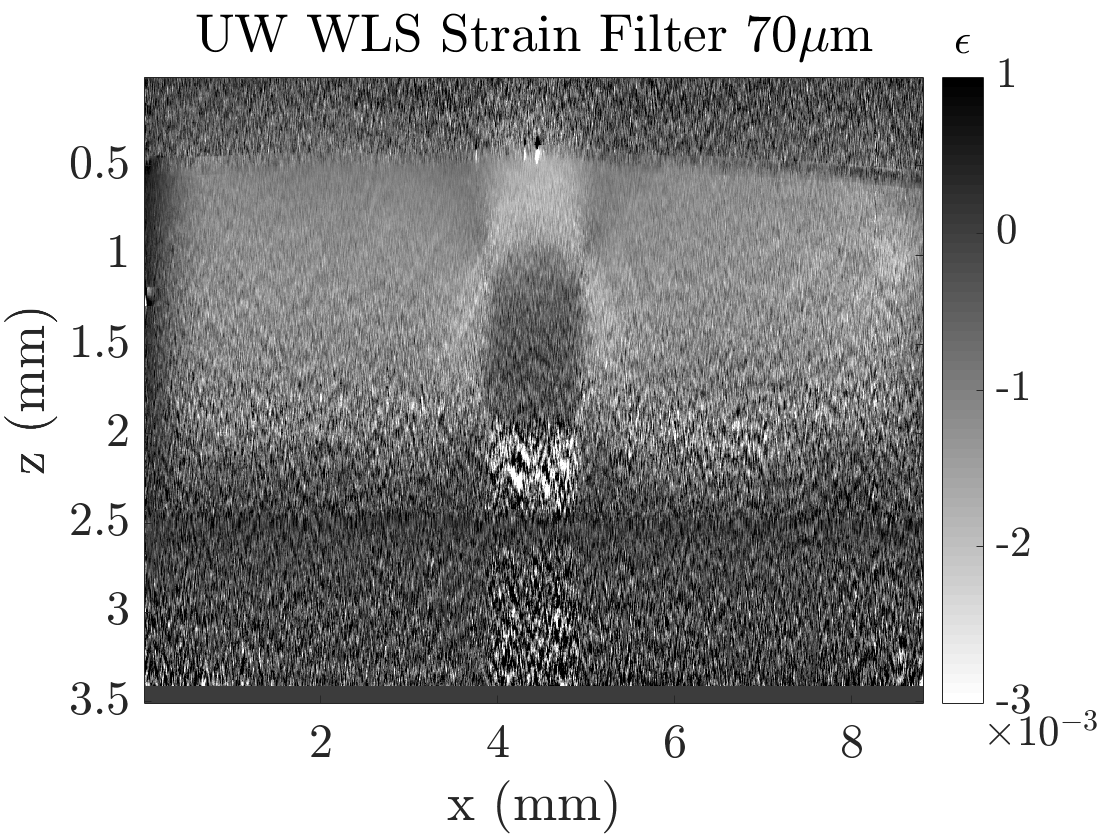
\includegraphics[width=\textwidth]{figures/wls_fr70_lr0.png}
	\end{subfigure}
    \begin{subfigure}{0.49\textwidth}
    	\centering
        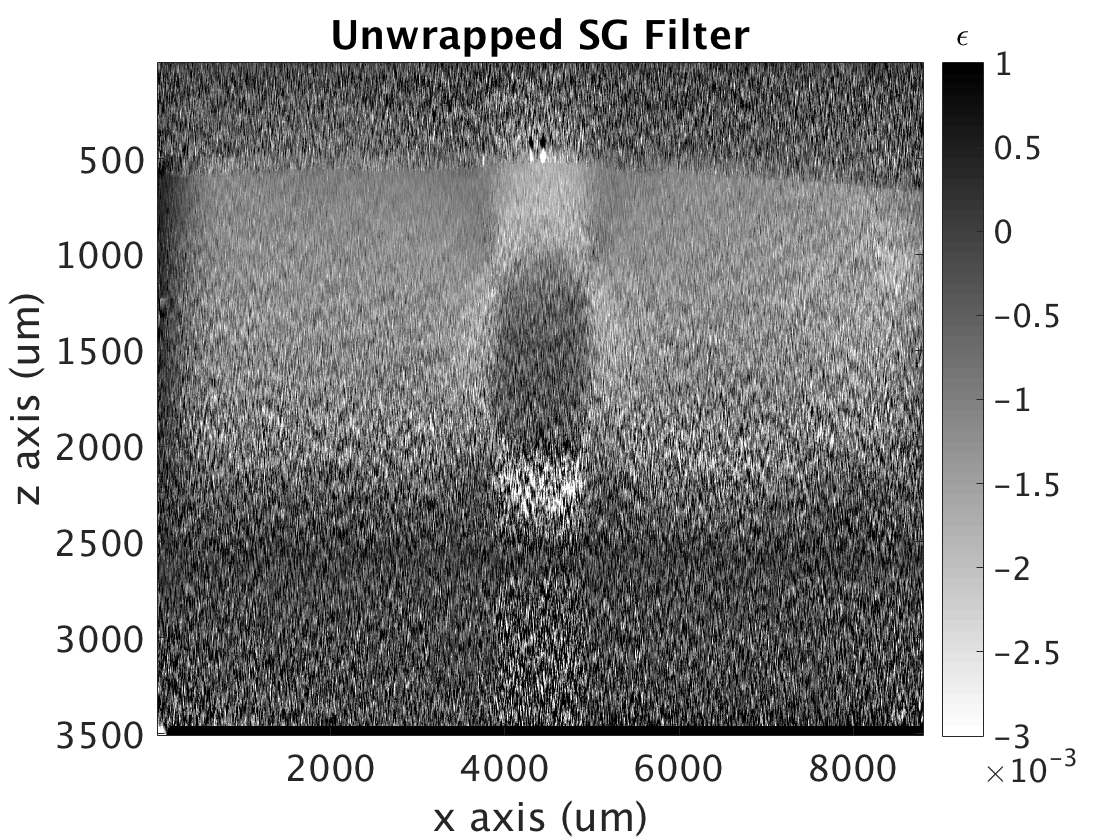
\includegraphics[width=\textwidth]{figures/uwsg_fr70_lr0.png}
	\end{subfigure}
    \\
    \begin{subfigure}{0.49\textwidth}
    	\centering
        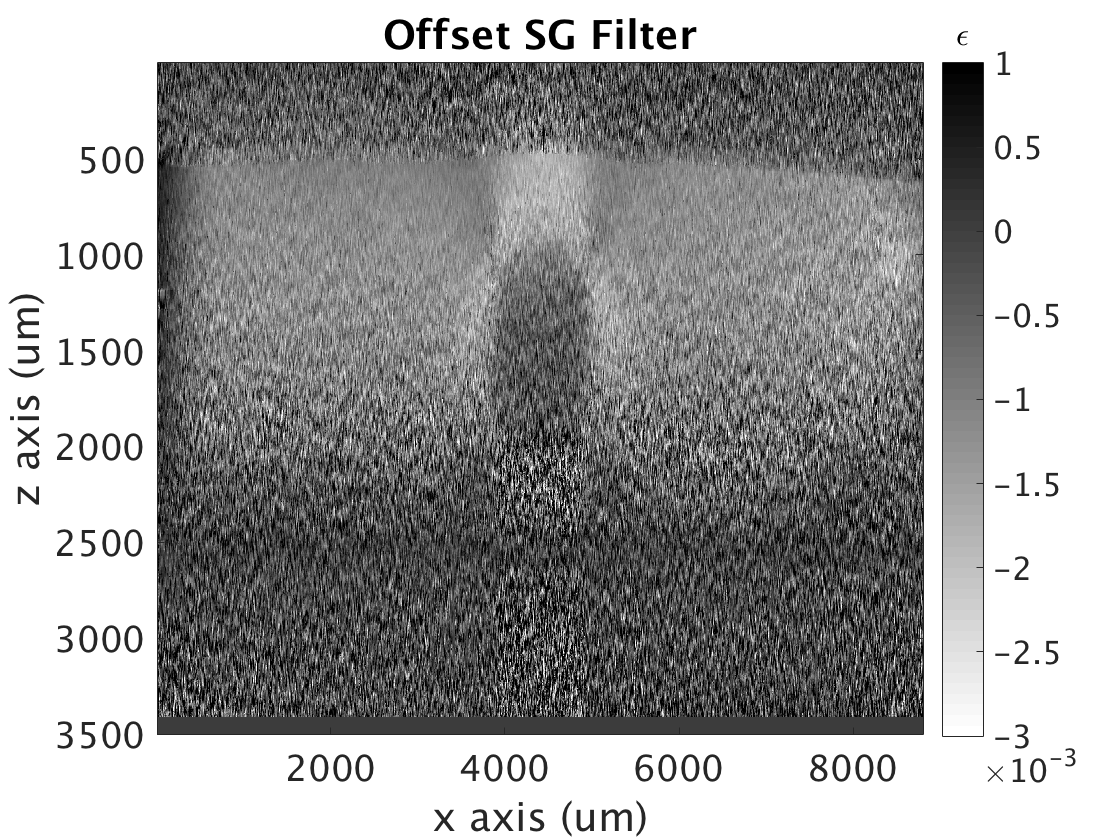
\includegraphics[width=\textwidth]{figures/posg_fr70_lr0.png}
	\end{subfigure}
    \begin{subfigure}{0.49\textwidth}
    	\centering
        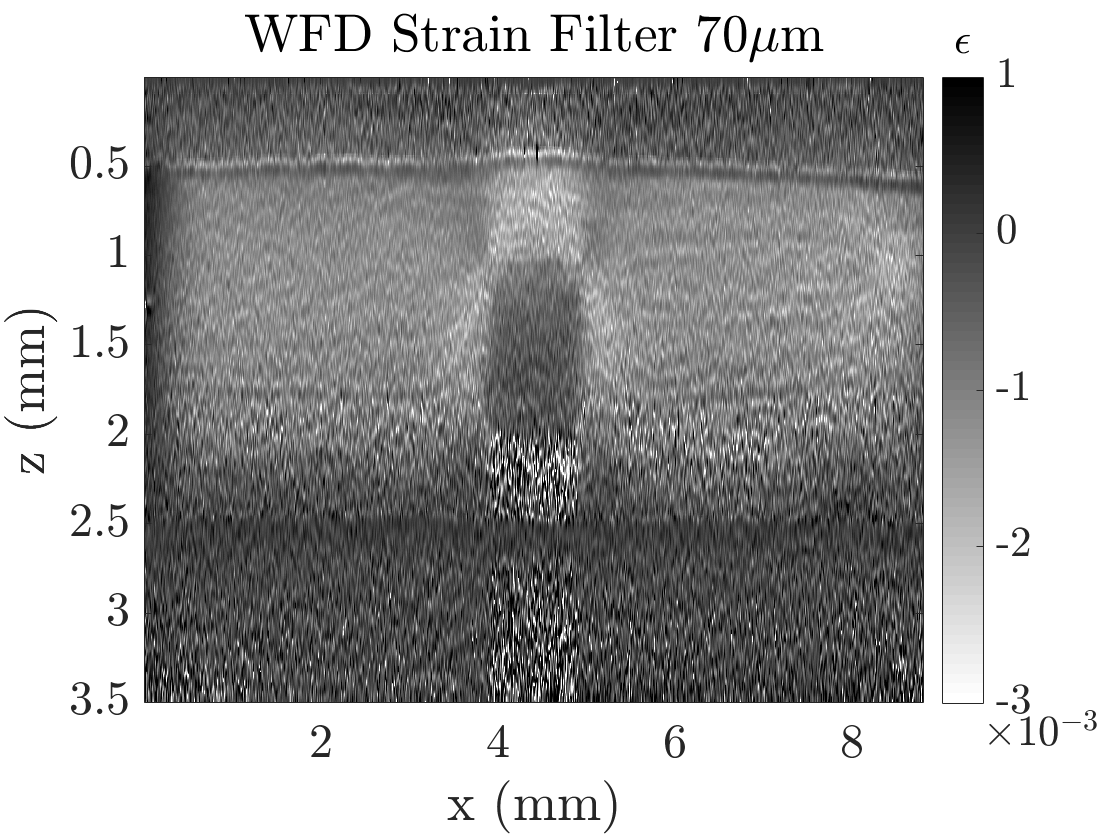
\includegraphics[width=\textwidth]{figures/wfd_fr70_lr0.png}
    \end{subfigure}
    \\
    \begin{subfigure}{0.49\textwidth}
    	\centering
        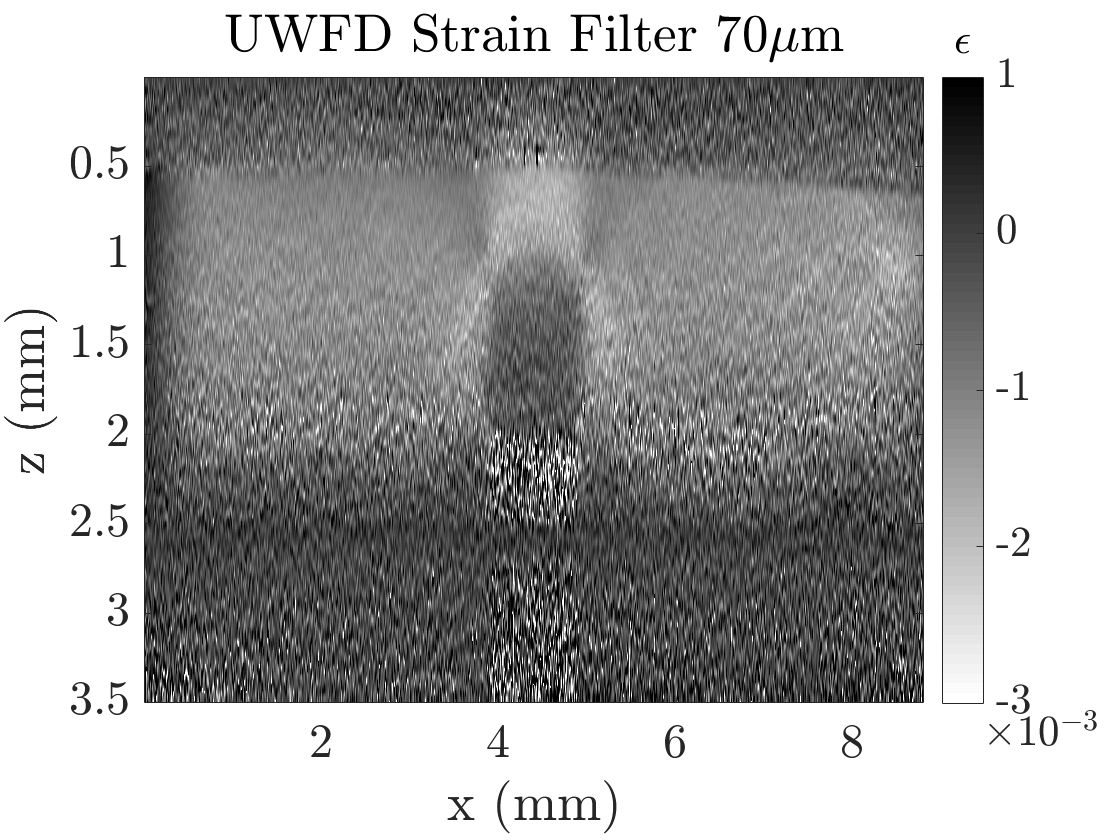
\includegraphics[width=\textwidth]{figures/uwfd_fr70_lr0.png}
	\end{subfigure}
    \begin{subfigure}{0.49\textwidth}
    	\centering
        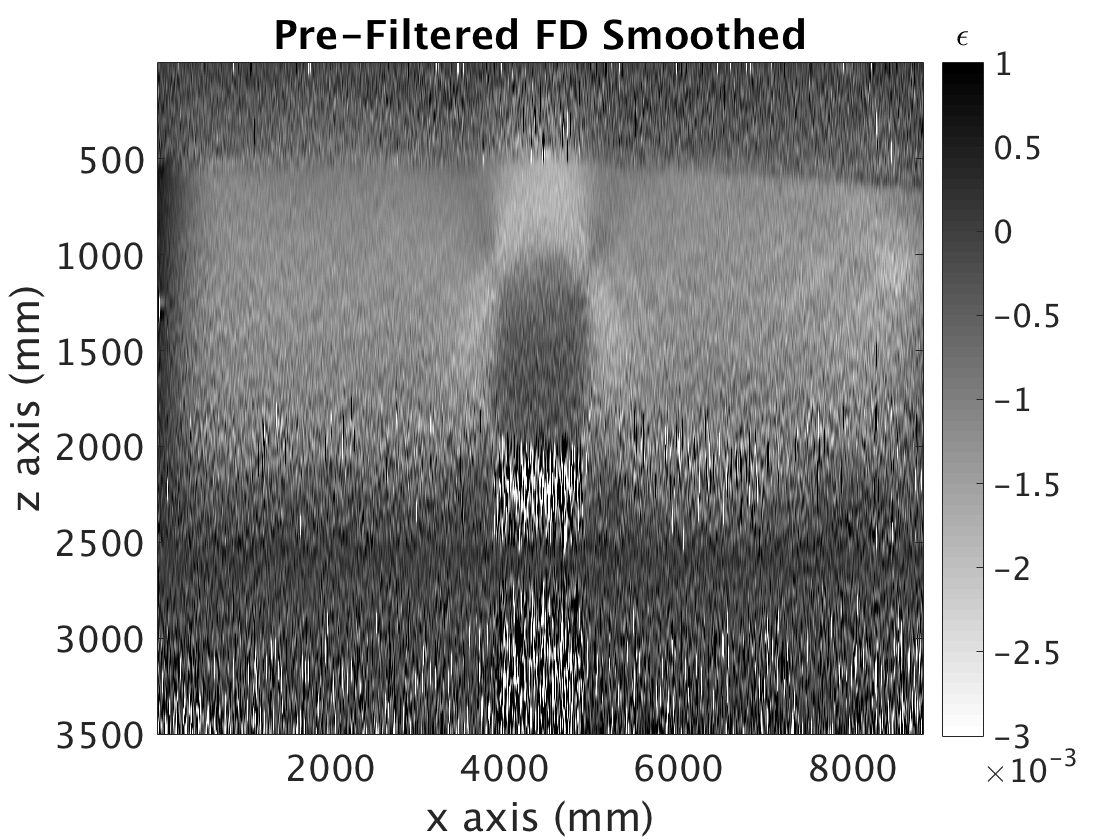
\includegraphics[width=\textwidth]{figures/fdsm_fr70_lr0.png}
    \end{subfigure}
    \caption{Strain B-scans taken from the centre of the phantom for the six strain estimation techniques discussed above. The strain values shown are windowed between -3 and 1 milli-strain.}
    \label{bscan_images_1}	
\end{figure}

\autoref{bscan_images_1} shows the resulting B-scan strain images, taken from the centre of the phantom, for the six different strain estimation techniques described above. Note that negative strain corresponds to compressive force, that is a displacement downwards. The fact that there exist positive strain values suggests that our assumption of uniaxial compression is invalid, as stiffer regions are pushing the softer bulk laterally and upwards. It can seen in all images that the stiff inclusion shows less strain than the softer surrounding bulk, as expected. There are similar 'halo' effects, caused by the stiff inclusion taking more of the compressive force than the soft bulk immediately next to it, in all images. The area under the hard inclusion is characterised by low OCT signal, as can be seen in \autoref{oct_image}, and is the most prominently noisy in the techniques that utilise a phase unwrapping algorithm over the entire volume, which is highly sensitive to strong fluctuations in OCT signal and as a result creates artefacts in these regions. A similar pattern is seen in this region in the weighted and unweighted smoothing of FD strain, and is very significant in the pre-filter FD image, which has in addition further streaks of strain estimation arguments at the bottom of the image. 

As mentioned before, the pre-filter FD with smoothed strain algorithm was introduced after noticing significant 'ripple' effects in the weighted smoothing of FD algorithm. These can be seen prominently to the top right of the inclusion, and match with features in the OCT image in \autoref{oct_image}. In addition to this, the surface of the sample, which has a high reflectance and therefore strong optical weighting, is a  prominent artefact in the weighted smoothing FD image. The application of a small pre-filter to this prior to smoothing appears to have removed this issue, as well as slightly decreased the impact of the optical features at the top right, however at the expense of introducing a multitude of streak artefacts into the bottom half of the image in areas of low OCT signal.

\subsection{Processing Time}


\begin{figure}[b!]
	\centering
    \begin{subfigure}{0.49\textwidth}
    	\centering
        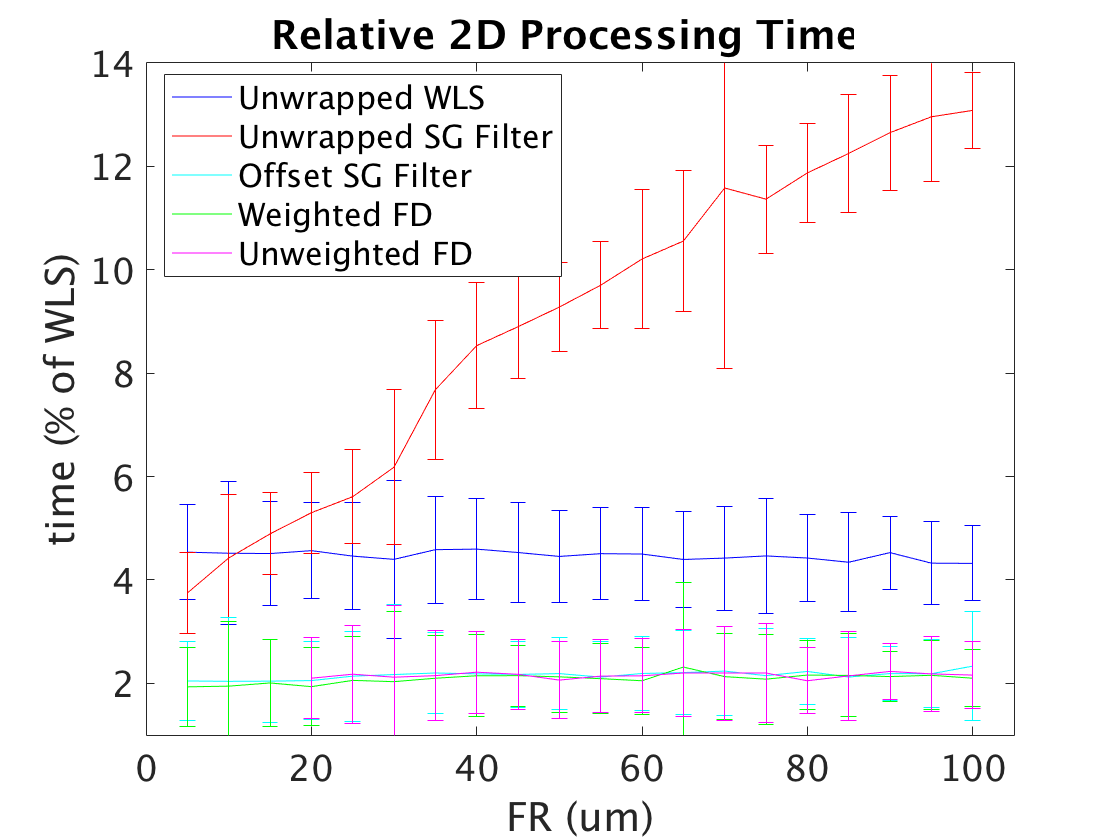
\includegraphics[width=\textwidth]{figures/2d_relative_fr.png}
    \end{subfigure}
    \begin{subfigure}{0.49\textwidth}
    	\centering
        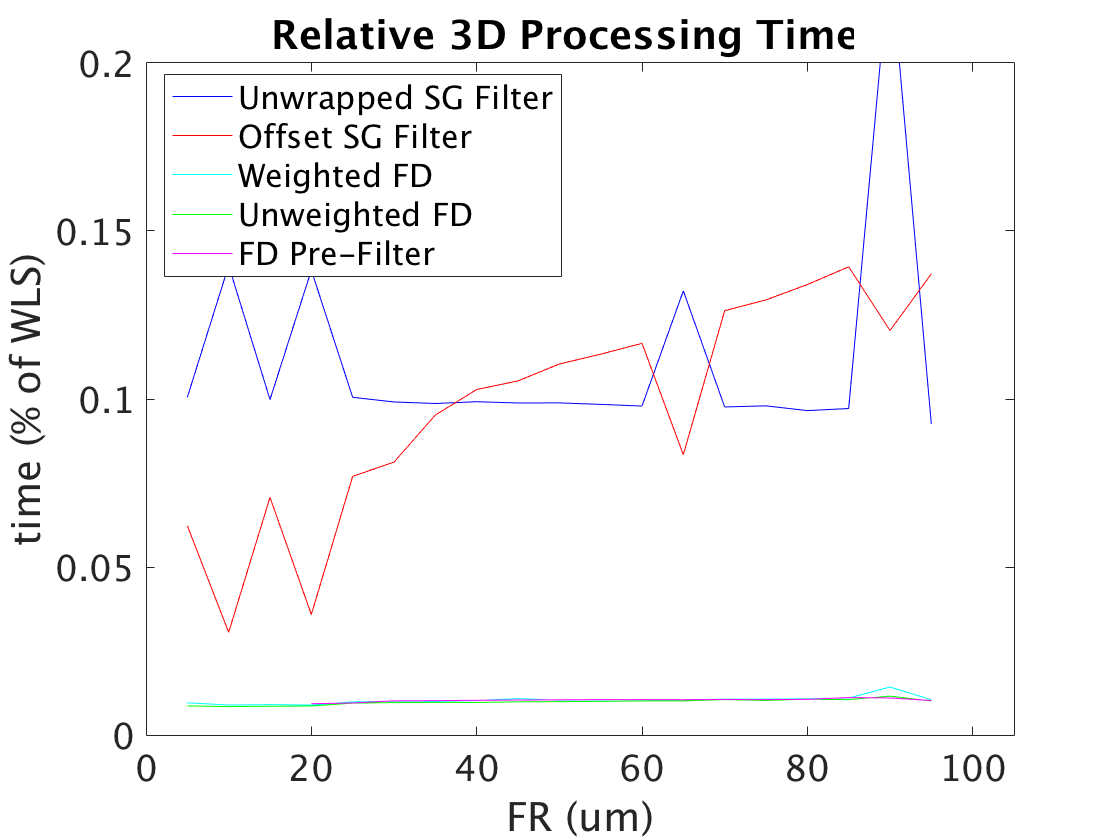
\includegraphics[width=\textwidth]{figures/3d_relative_fr.png}
    \end{subfigure}
    \caption{Relative processing time for different strain estimation techniques at different fit resolution values for a) a single B-scan and b) an entire C-scan. Error bars are the standard deviation of 50 repeated measurements.}
    \label{process_time_1}
\end{figure}

\autoref{process_time_1} shows the relative processing time for the different strain estimation techniques for both a single @D B-scan and an entire 3D C-scan, at different fit resolutions. Note that in order to compare accurately between the 2D B-scan and C-scan, a 2D unwrapping algorithm was implemented instead of the usual 3D that laterally unwraps as well. Each data point corresponds to an average of 50 processing time measurements. The error bars in the plot are the standard deviations of these 50 measurements. Since this is plotted relatively, the standard deviation of the relative measurement is equal to the addition of the standard deviations of the absolute measurement and the baseline (WLS) measurement.

The relative processing time (with respect to the WLS with unwrapped phase) is shown instead of the actual, to try provide an estimate that is comparable across different machines.

It can be seen that all new strain estimation techniques show a significant improvement in processing speed compared to the WLS estimate. In particularly, the finite difference techniques are particularly fast. The Savitzky-Golay filter on the unwrapped phase is faster than when applied to the phase offset, suggesting that the bottleneck caused by the non-linear subtraction operation contributes more to slowing the process down than needing to perform unwrapping on the entire volume. 

\subsection{Sensitivity}

\begin{figure}[b!]
	\centering
    \begin{subfigure}{0.49\textwidth}
    	\centering
        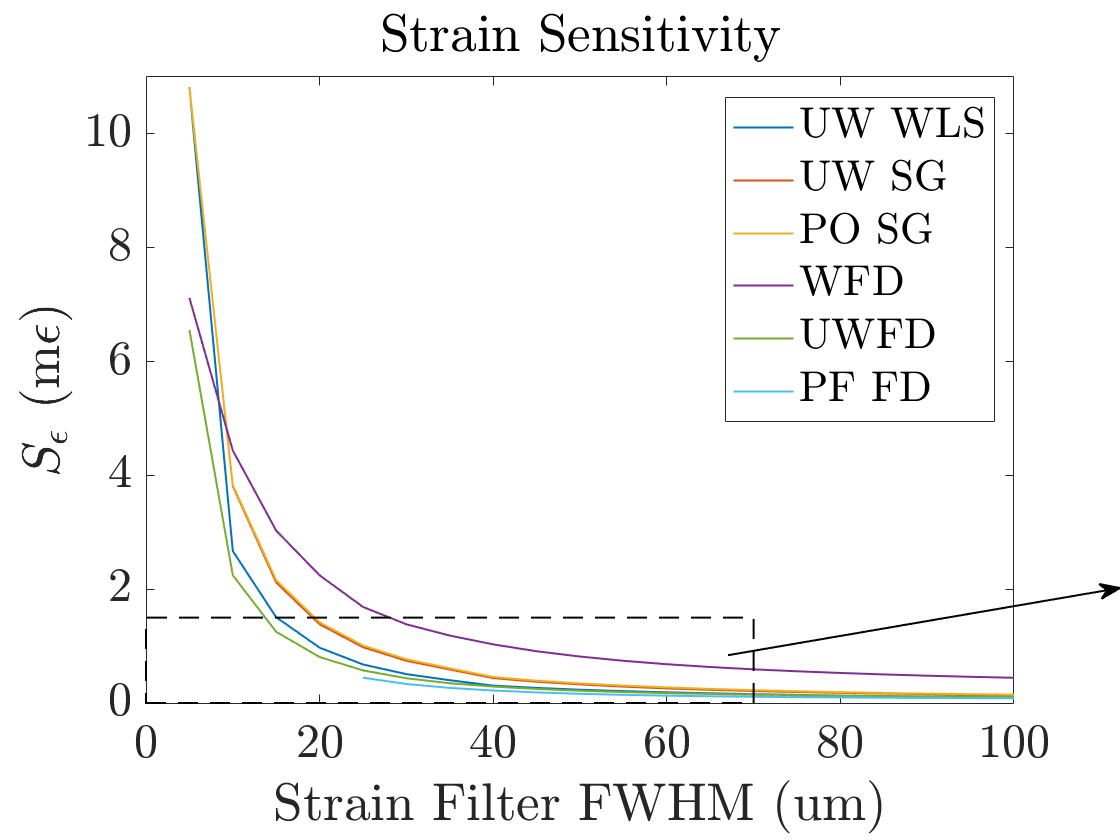
\includegraphics[width=\textwidth]{figures/sensitivity_lr0_arrow.png}
    \end{subfigure}
    \begin{subfigure}{0.49\textwidth}
    	\centering
        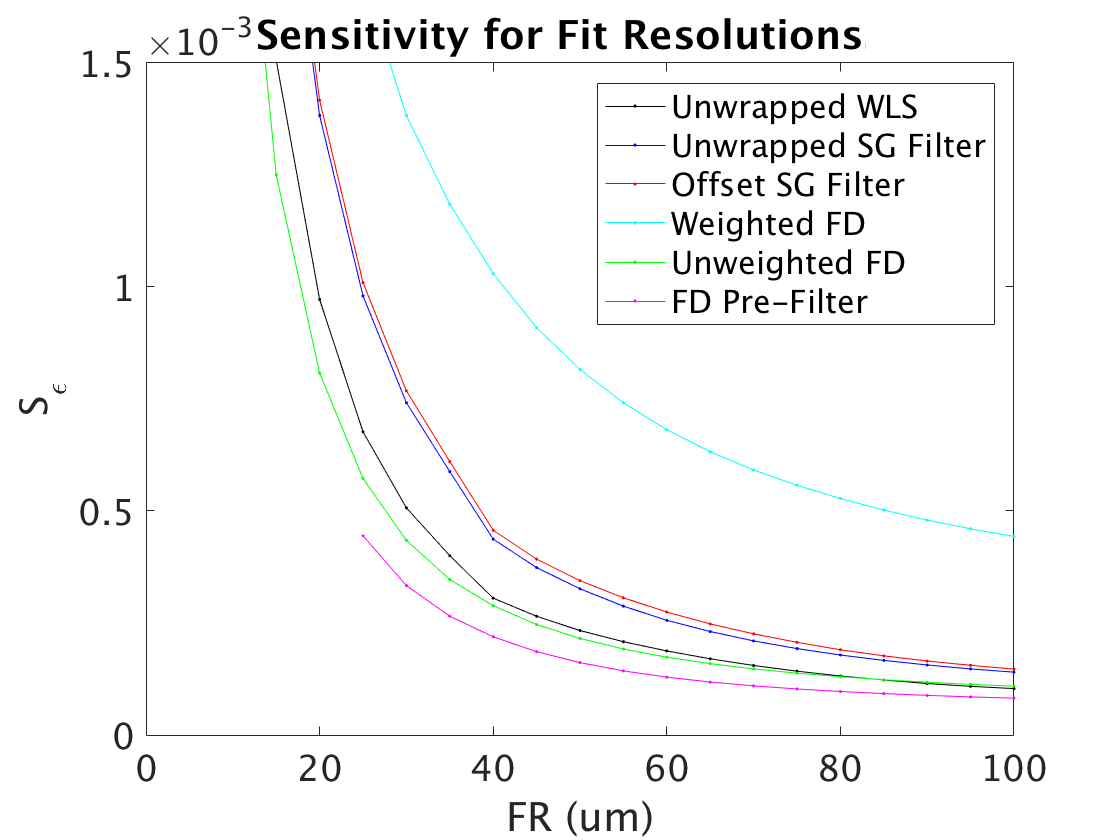
\includegraphics[width=\textwidth]{figures/sensitivity_lr0_zoom.png}
    \end{subfigure}
    \caption{Strain sensitivity values at different fit resolutions for all strain estimation techniques. The plot on the left is zoomed in to show the differences more clearly.}
	\label{sensitivity_1}
\end{figure}

The strain sensitivity for the six different estimation techniques for different fit resolutions is shown in \autoref{sensitivity_1}. There is a clear trend across all techniques, that at the larger fit resolutions the sensitivity is better. The downside of this is that at larger fit resolutions, the ability to distinguish objects laterally is significantly worsened, as can be seen in strain B-scan images in \autoref{strain_bscan_images}. Therefore there is a need to optimise the trade off between sensitivity and fit resolution. The three techniques that offer the best sensitivity at lower fit resolutions are WLS, unweighted smoothing with FD, and the pre-filtered FD. Note that the weighted smoothing with FD is significantly worse than the other techniques, due to the artefacts discussed above. The phase offset and unwrapping with SG filtering are slightly worse than the WLS estimate, likely due to them being an ordinary least squares estimate, as opposed to a weighted one.

Although the pre-filtered FD supposedly shows the best sensitivity, it is important to note the artefacts present in the qualitative evaluation of the image. Therefore this sensitivity measurement is not indicative of the image quality as a whole, but only a segment of it.

On the basis of these results, it was decided to see if implementing lateral averaging over the separated B-scans could improve the sensitivity of the lower-order differentiation techniques (in particular the weighted FD and the SG filtering) towards that of the WLS. 

\section{Phantom Strain Elastogram Results with Lateral Averaging}\label{phantom_results_lateral}

\subsection{Qualitative Comparison}
It was found that very comparable image quality could be achieved using a smaller fit resolution of $40\mu m$ when lateral smoothing was also applied. \autoref{images} contains the B-scan  images for the different strain estimation techniques for selected fit resolution and lateral resolution values. 

\subsection{Processing Time}
The benefit of adding lateral averaging is that it improves the sensitivity, and in most instances, without adding much time overhead, since it can be implemented as a 2D convolution on a given B-scan. Therefore the focus of this section is mostly on the image quality, rather than the processing time. However, \autoref{process_time_2} shows that adding lateral smoothing did not change the relative positions of the processing techniques in terms of processing time.

\begin{figure}[th!]
	\centering
    \begin{subfigure}{0.49\textwidth}
    	\centering
        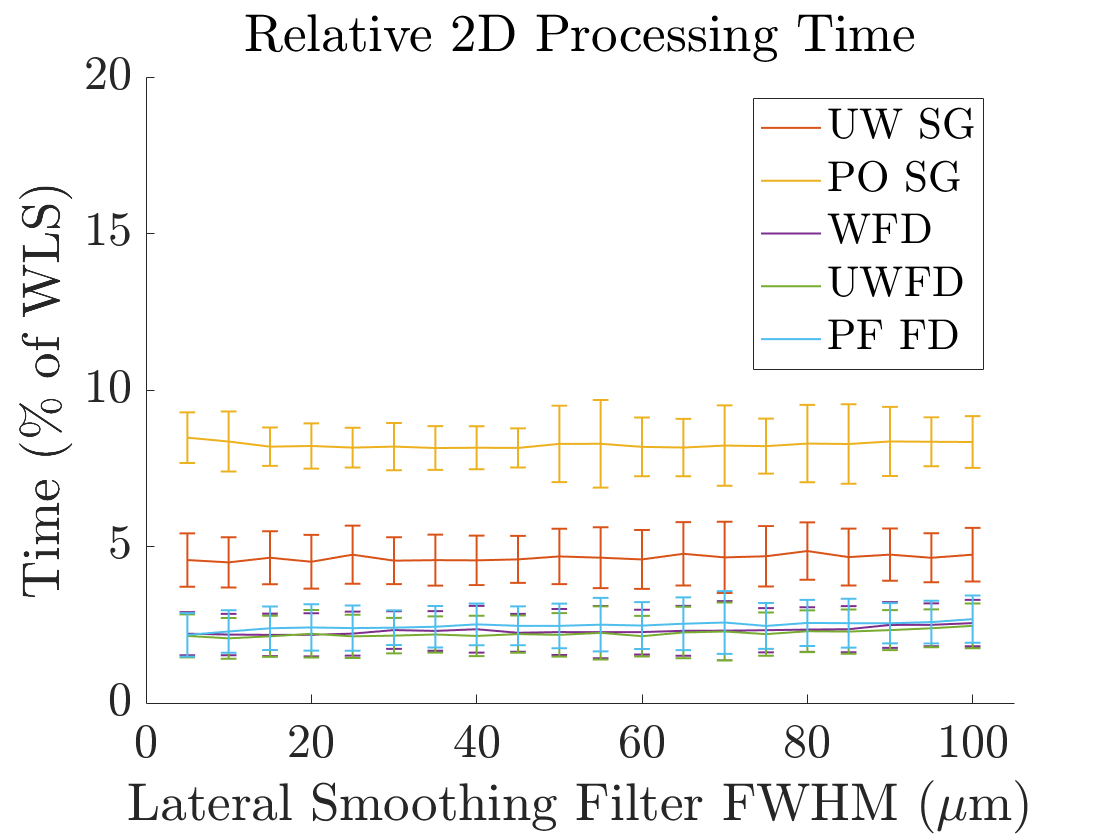
\includegraphics[width=\textwidth]{figures/2d_relative_lr.png}
    \end{subfigure}
    \begin{subfigure}{0.49\textwidth}
    	\centering
        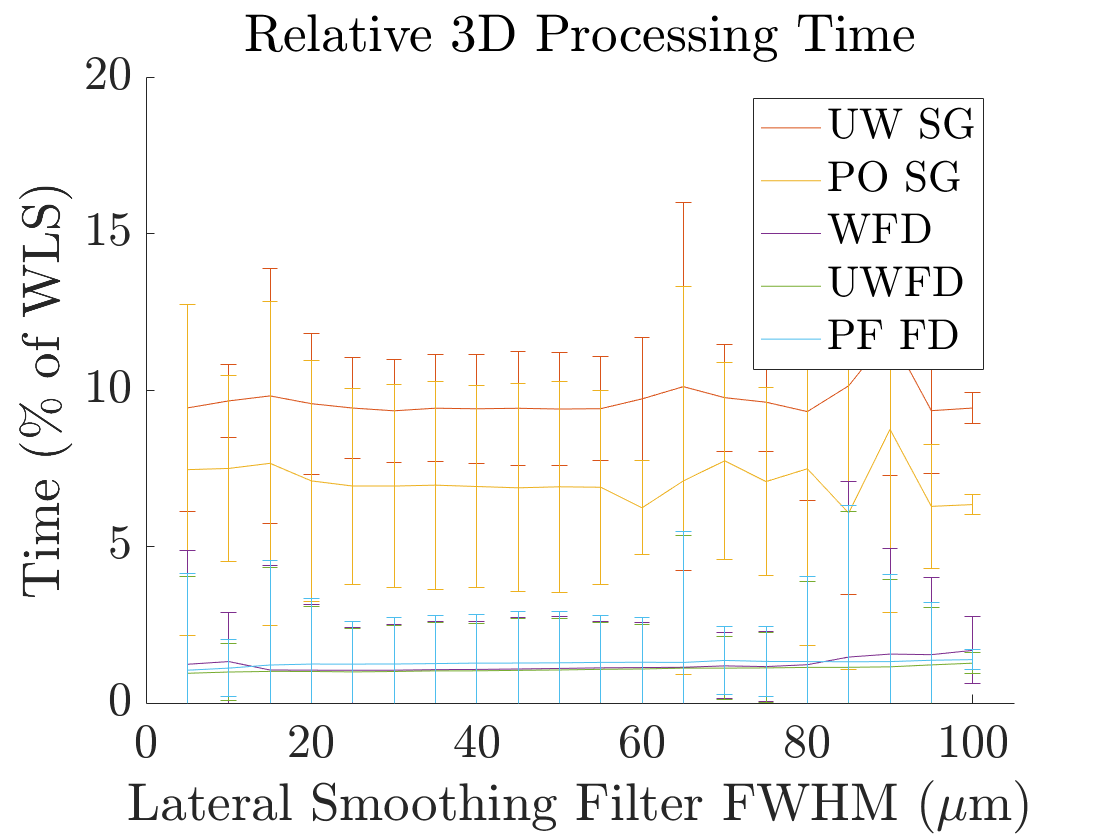
\includegraphics[width=\textwidth]{figures/3d_relative_lr.png}
    \end{subfigure}
    \caption{Relative processing time for different strain estimation techniques at a fit resolution of $40\mu m$ and with different lateral smoothing resolutions for a) a single B-scan and b) an entire C-scan.}
    \label{process_time_2}
\end{figure}

\subsection{Sensitivity}

The addition of lateral smoothing heightens the sensitivity of all imaging techniques. At the standard fit resolution, \autoref{sensitivity_2} shows significant improvement in the sensitivity when lateral smoothing is applied, for all techniques.

\begin{figure}[b!]
	\centering
    \begin{subfigure}{0.49\textwidth}
    	\centering
        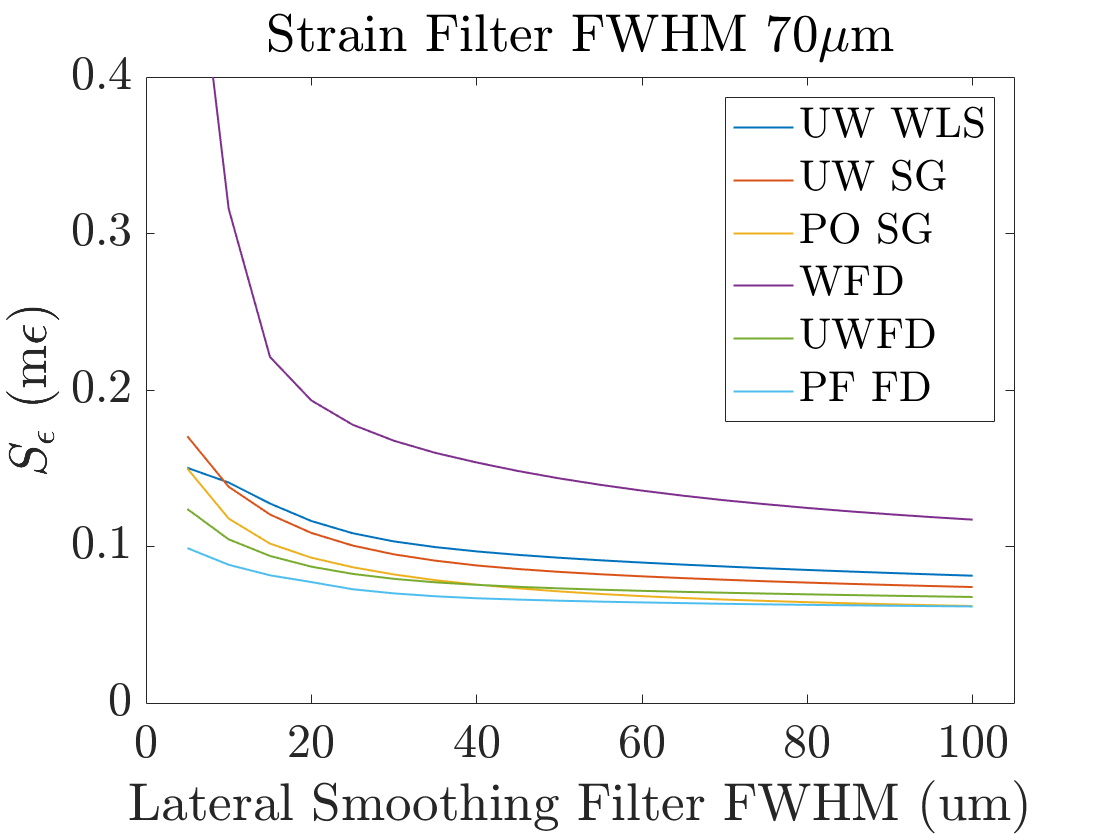
\includegraphics[width=\textwidth]{figures/sensitivity_fr70.png}
    \end{subfigure}
    \begin{subfigure}{0.49\textwidth}
    	\centering
        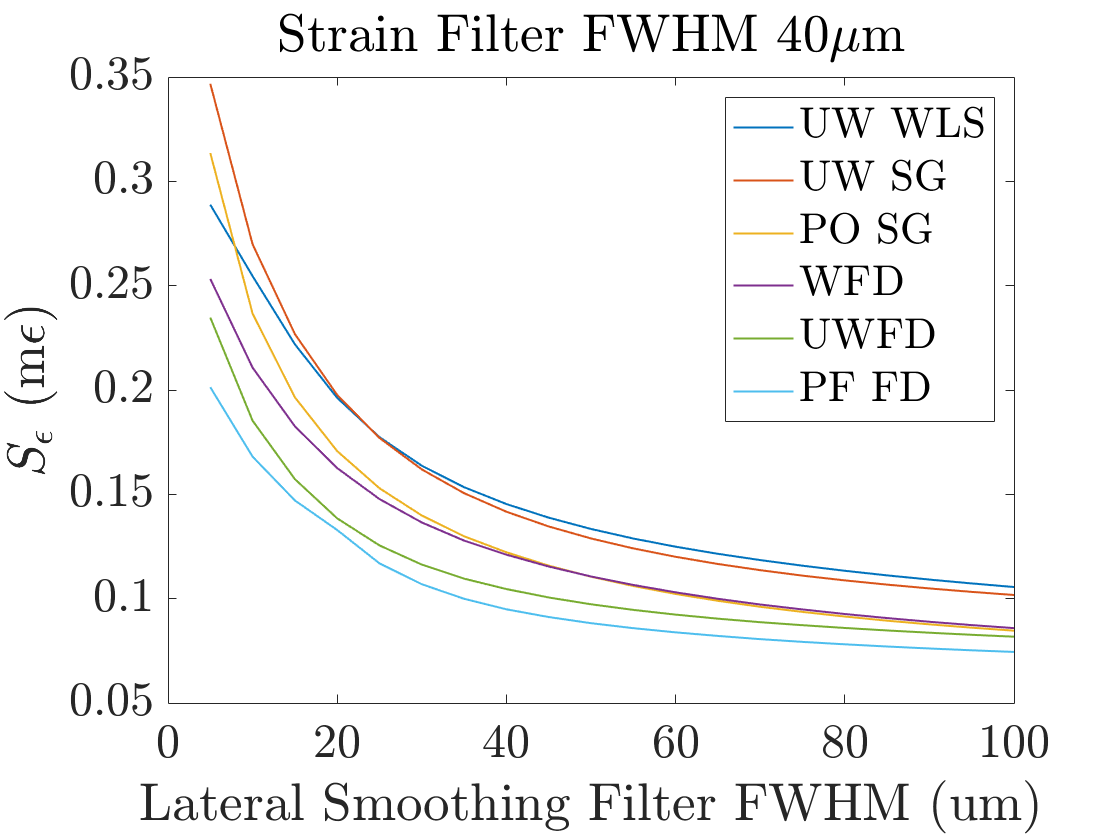
\includegraphics[width=\textwidth]{figures/sensitivity_fr40.png}
    \end{subfigure}
    \caption{Strain sensitivity for different lateral smoothing resolutions for a) Fit resolution of $70\mu m$, and b) $40\mu m$.}
    \label{sensitivity_2}	
\end{figure}


\begin{table}[h]
	\begin{center}
		\begin{tabular}{|c c|c c c c c c|}
			\hline 
			SF FWHM & LSF FWHM & UW WLS & UW SG & PO SG & WFD & UWFD & PF FD \\
			\hline
			\hline
			40 & 0 & 0.320 & 0.437 & 0.457 & 0.287 & 0.289 & 0.219 \\
			70 & 0 & 0.161 & 0.256 & 0.274 & 0.215 & 0.174 & 0.129 \\
			100 & 0 & 0.107 & 0.140 & 0.147 & 0.171 & 0.109 & 0.082 \\
			40 & 20 & 0.196 & 0.198 & 0.171 & 0.163 & 0.139 & 0.133 \\
			70 & 20 & 0.108 & 0.109 & 0.096 & 0.125 & 0.088 & 0.079 \\
			100 & 20 & 0.079 & 0.088 & 0.071 & 0.107 & 0.077 & 0.069 \\
			40 & 40 & 0.145 & 0.142 & 0.122 & 0.121 & 0.105 & 0.095 \\
			70 & 40 & 0.089 & 0.088 & 0.077 & 0.096 & 0.076 & 0.068 \\
			100 & 40 & 0.069 & 0.077 & 0.059 & 0.081 & 0.071 & 0.063 \\
			\hline
		\end{tabular}
	\end{center}
	\caption{Strain sensitivity values (given in m$\epsilon$) for selected strain filter (SF) FWHM and lateral smoothing filter (LSF) FWHM, given in $\mu$m. The six strain estimation techniques are ordered as defined above in \autoref{algorithms}.}
	\label{sensitivity_table}
\end{table}

\autoref{sensitivity_table} shows the sensitivity results for selected combinations of fit and lateral resolutions, for which the images themselves are shown in \autoref{images}.

It has been shown that it is possible to greatly reduce the processing time by using finite difference approaches, and that the sensitivity can be optimised by introducing lateral smoothing, which can be computed very quickly using a convolution operation. However, the image is not infinitely improved with more lateral smoothing and higher fit resolutions. The degradation of the image resolution, due to these processes, must be examined. 

\section{Analysis of Image Resolution} \label{image_res_results}

A goodness of fit limit was placed on the process of fitting an error function to the data set in order to calculate the image resolution, by requiring that the R-squared value of the fit must be over 0.5, which is quite low. However by visually examining the fits made, it was found that the high amounts of noise in the strain filter and lateral filters with low FWHM degraded the R-squared value, however visual inspection showed a fit that was still reasonably followed the data trend. Using these filtered results, it was found that the process of fitting a step response to the object boundaries was impossible for strain elastograms with no lateral smoothing and for very low strain filtering resolutions, due to the high frequency noise corrupting the data. \autoref{imageres_figs} show density plots of the axial and lateral image resolution FWHM for the different strain estimation techniques.

\begin{figure}[hb!]
	\centering
	\begin{subfigure}{0.49\textwidth}
		\centering
		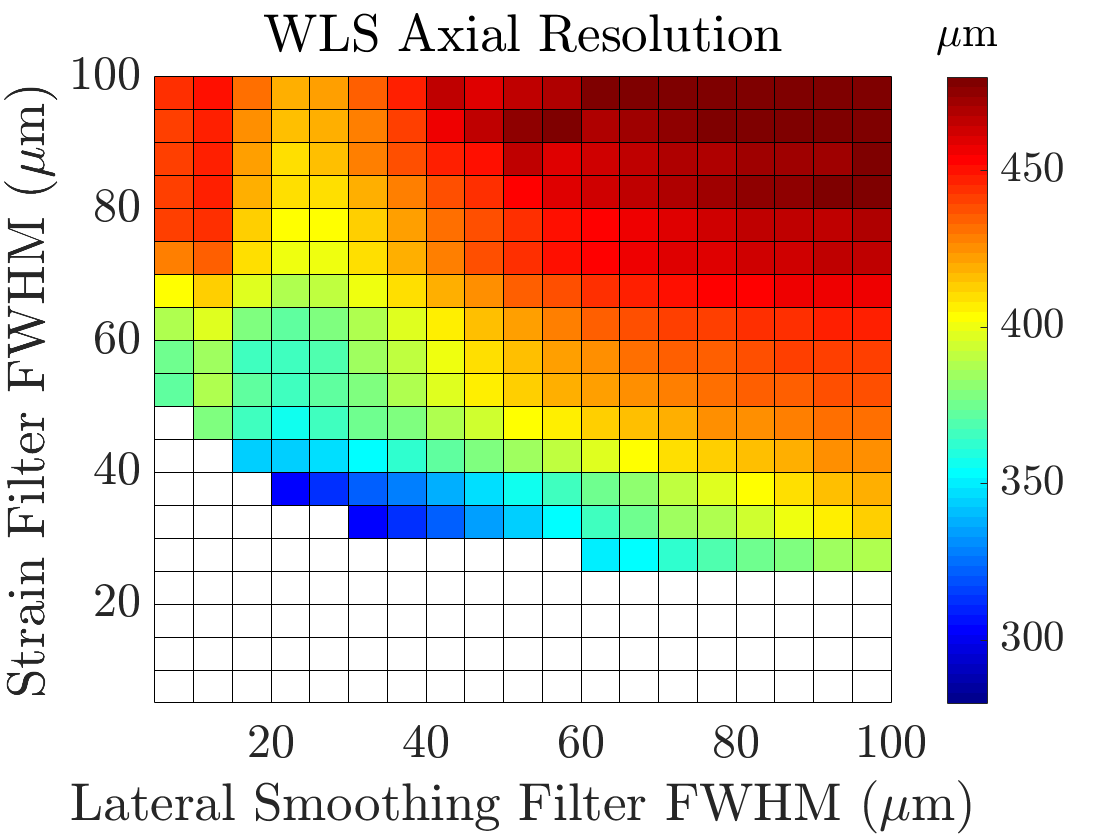
\includegraphics[width=\textwidth]{imageres_figs/wls_axial.png}
	\end{subfigure}
	\begin{subfigure}{0.49\textwidth}
		\centering
		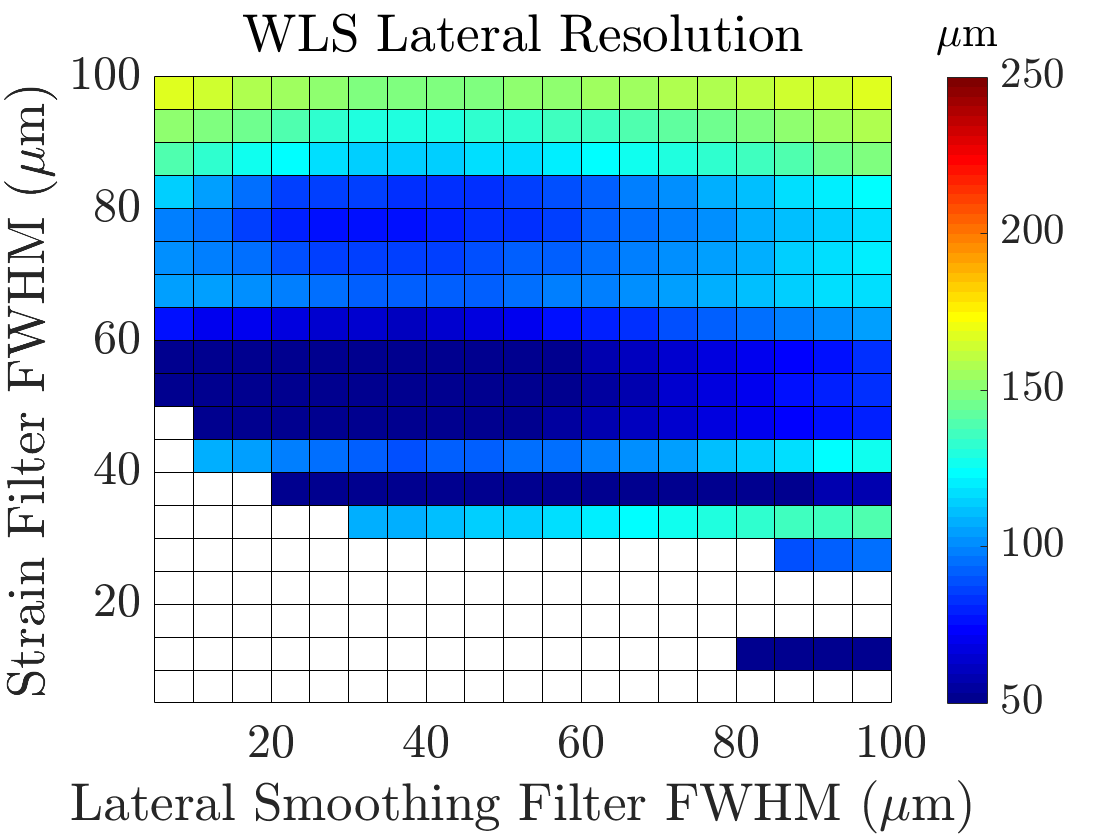
\includegraphics[width=\textwidth]{imageres_figs/wls_lateral.png}
	\end{subfigure}
	\\
	\begin{subfigure}{0.49\textwidth}
		\centering
		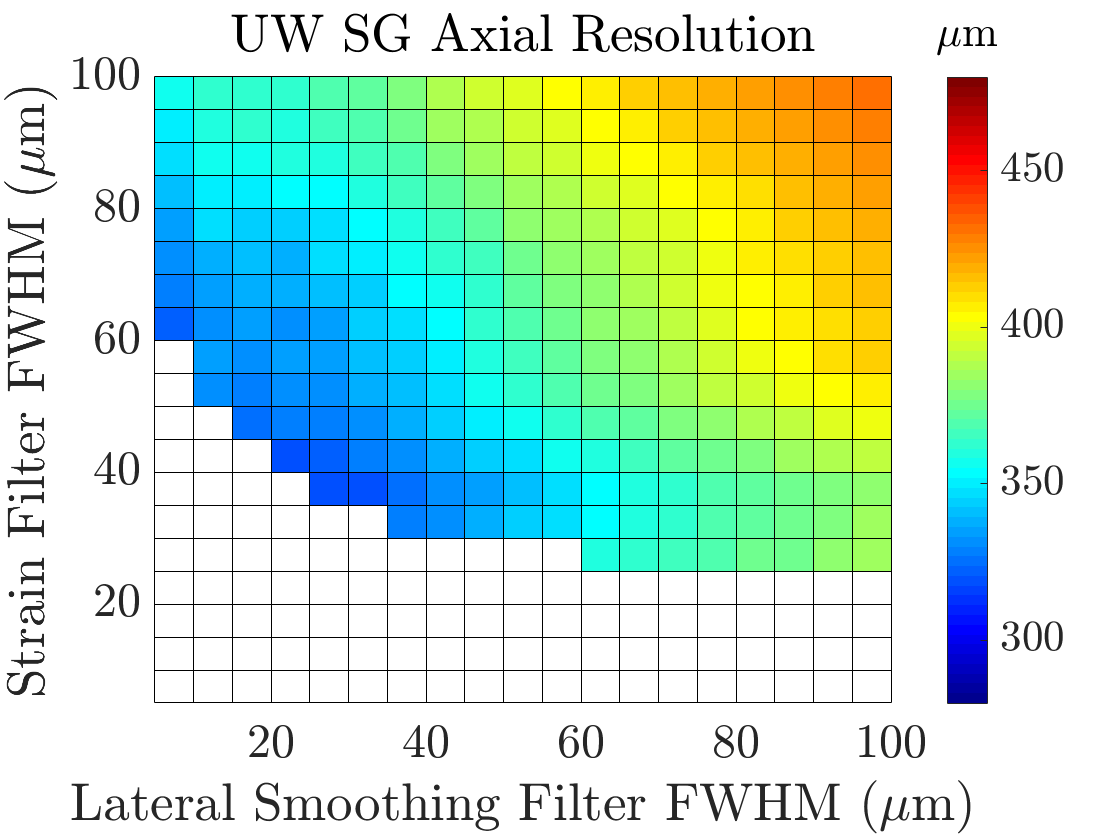
\includegraphics[width=\textwidth]{imageres_figs/uwsg_axial.png}
	\end{subfigure}
	\begin{subfigure}{0.49\textwidth}
		\centering
		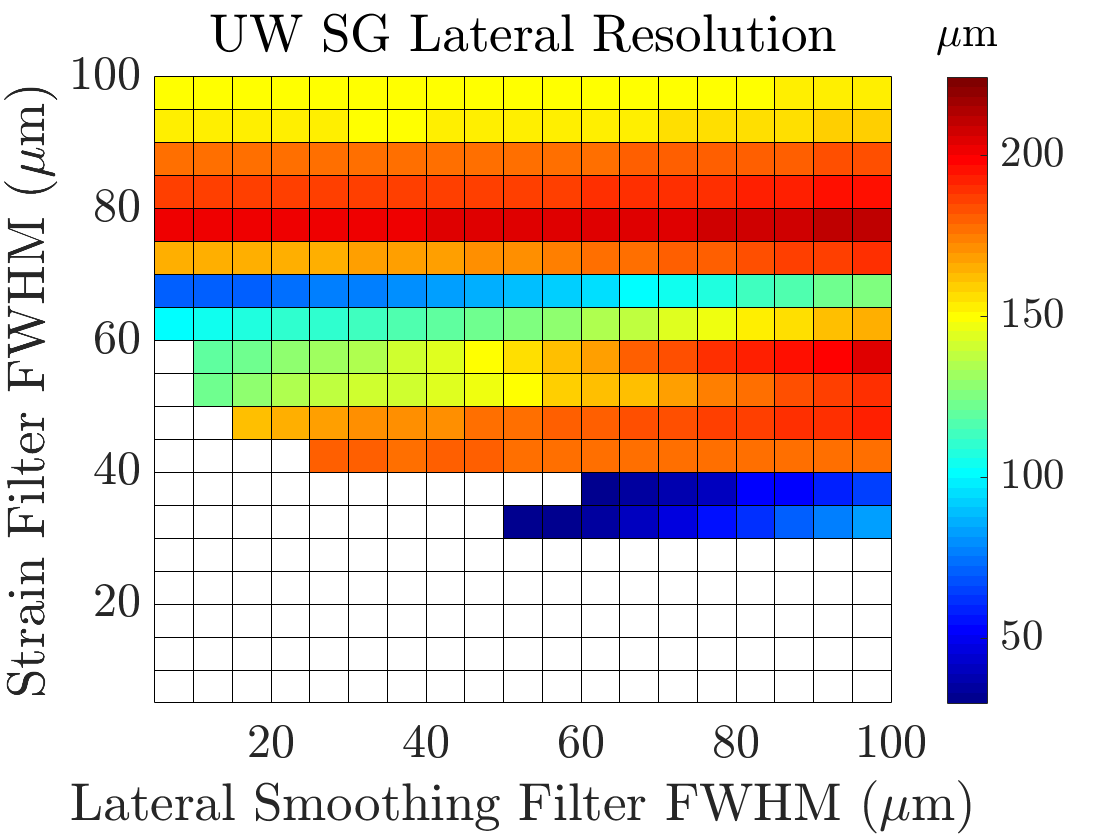
\includegraphics[width=\textwidth]{imageres_figs/uwsg_lateral.png}
	\end{subfigure}
\end{figure}
\begin{figure}[htb]\ContinuedFloat
		\begin{subfigure}{0.49\textwidth}
		\centering
		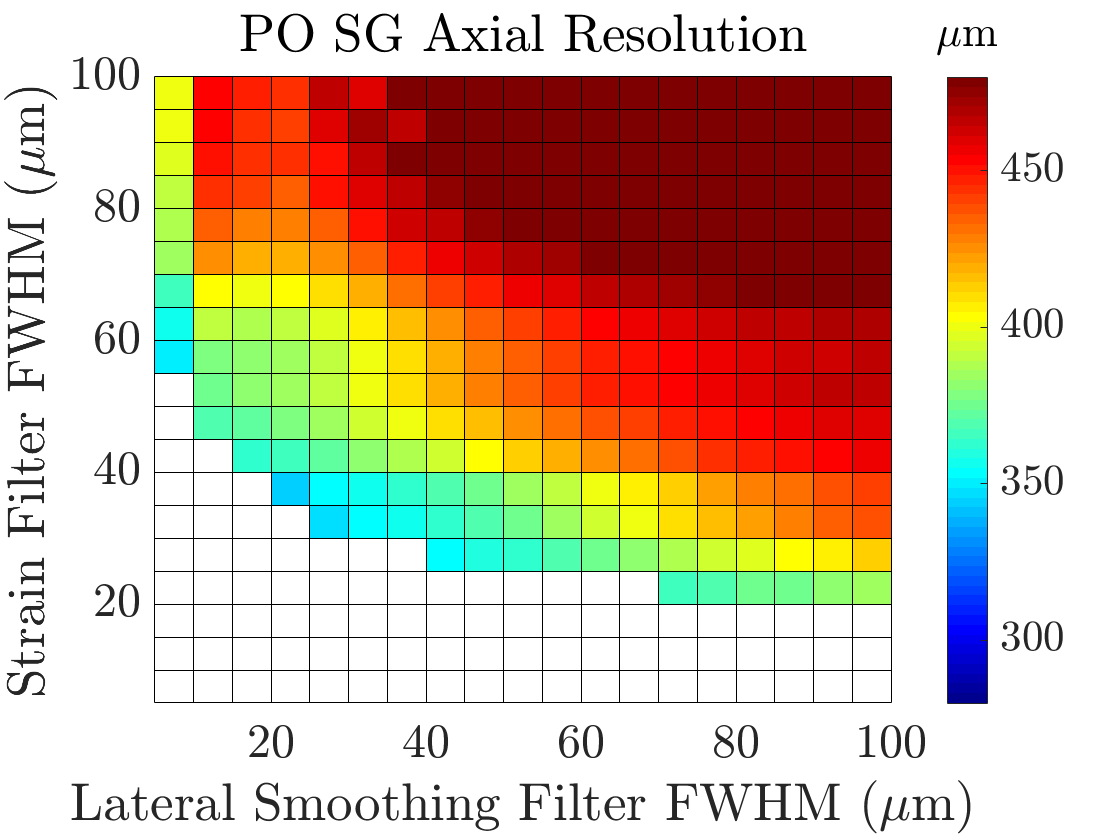
\includegraphics[width=\textwidth]{imageres_figs/posg_axial.png}
	\end{subfigure}
	\begin{subfigure}{0.49\textwidth}
		\centering
		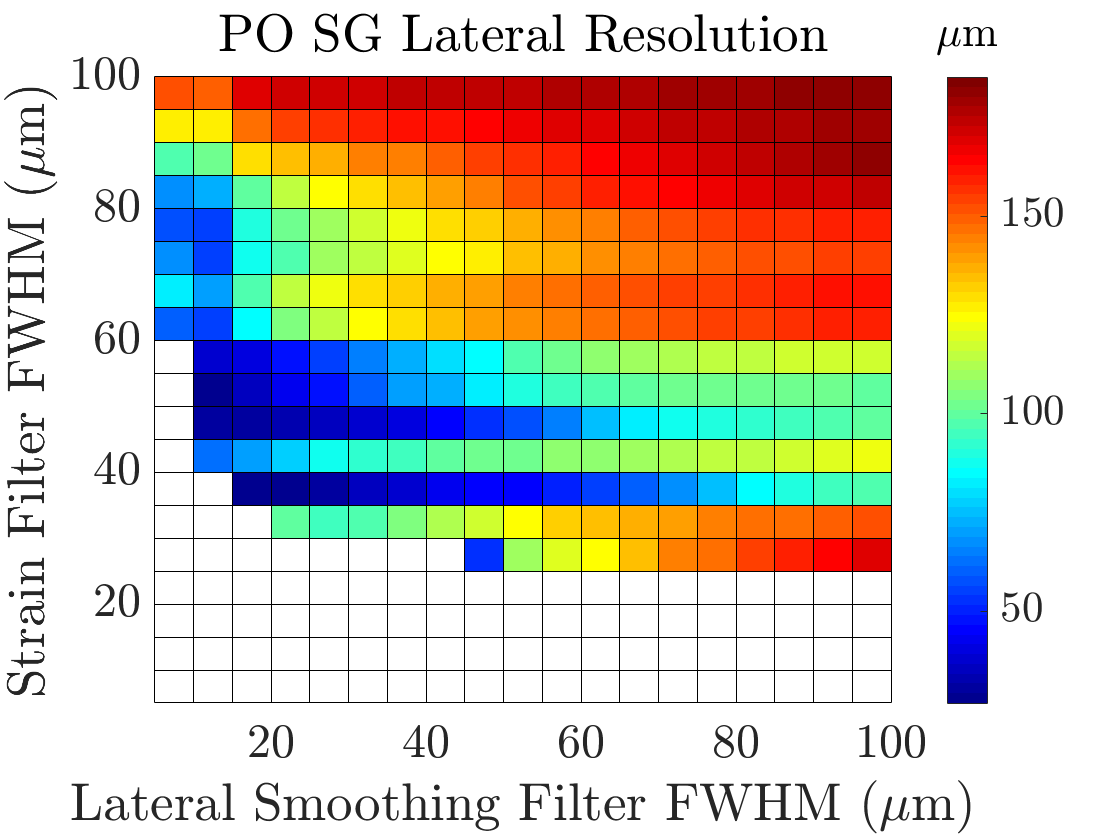
\includegraphics[width=\textwidth]{imageres_figs/posg_lateral.png}
	\end{subfigure}
	\\
	\begin{subfigure}{0.49\textwidth}
		\centering
		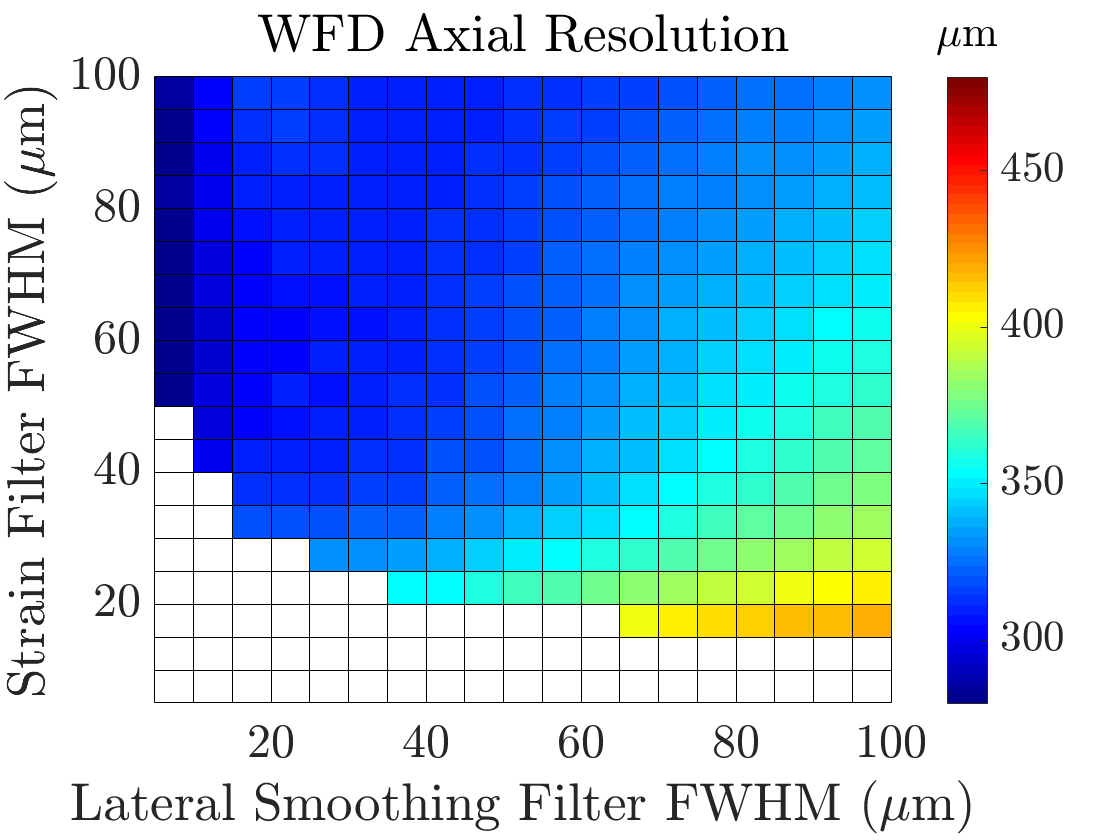
\includegraphics[width=\textwidth]{imageres_figs/wfd_axial.png}
	\end{subfigure}
	\begin{subfigure}{0.49\textwidth}
		\centering
		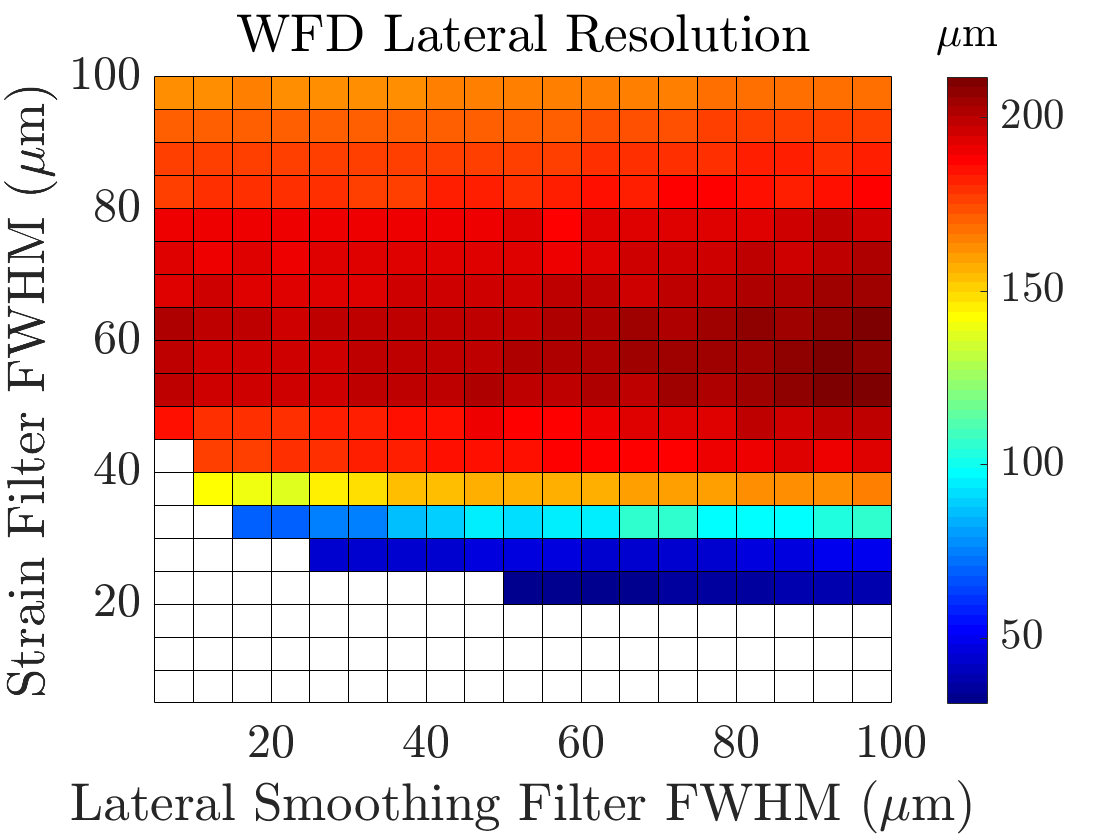
\includegraphics[width=\textwidth]{imageres_figs/wfd_lateral.png}
	\end{subfigure}
	\\
	\begin{subfigure}{0.49\textwidth}
		\centering
		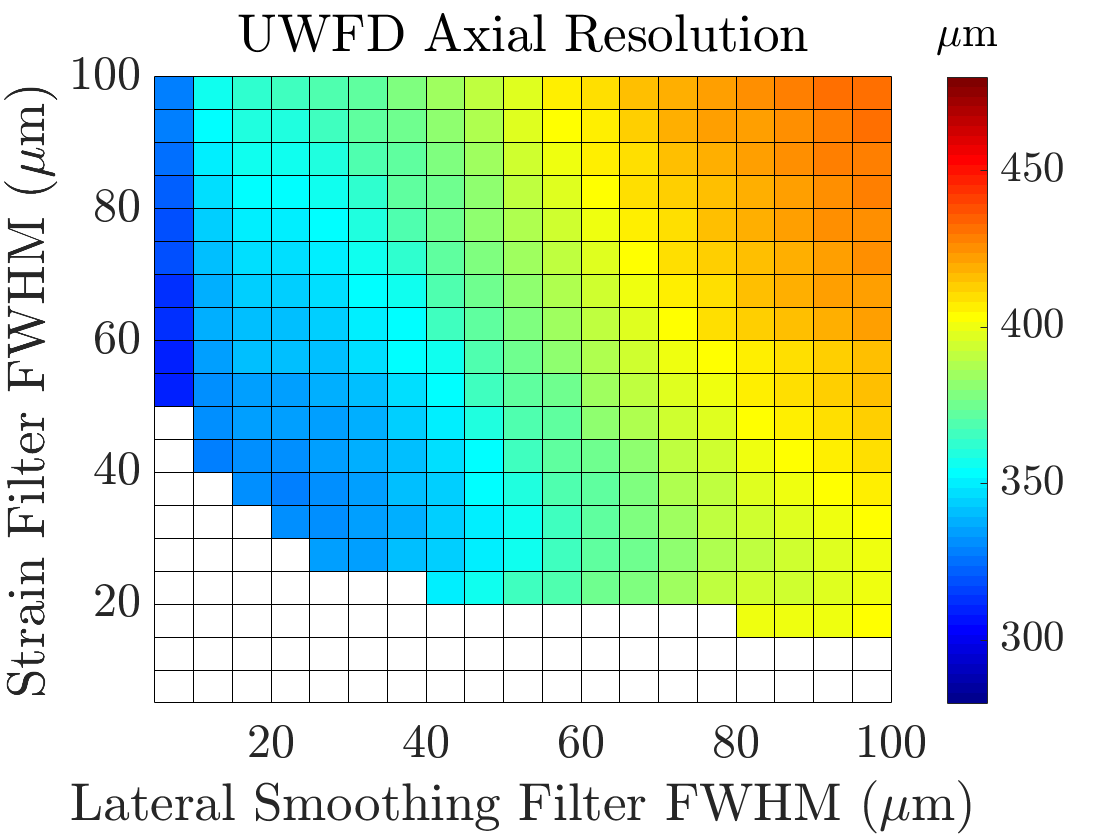
\includegraphics[width=\textwidth]{imageres_figs/uwfd_axial.png}
	\end{subfigure}
	\begin{subfigure}{0.49\textwidth}
		\centering
		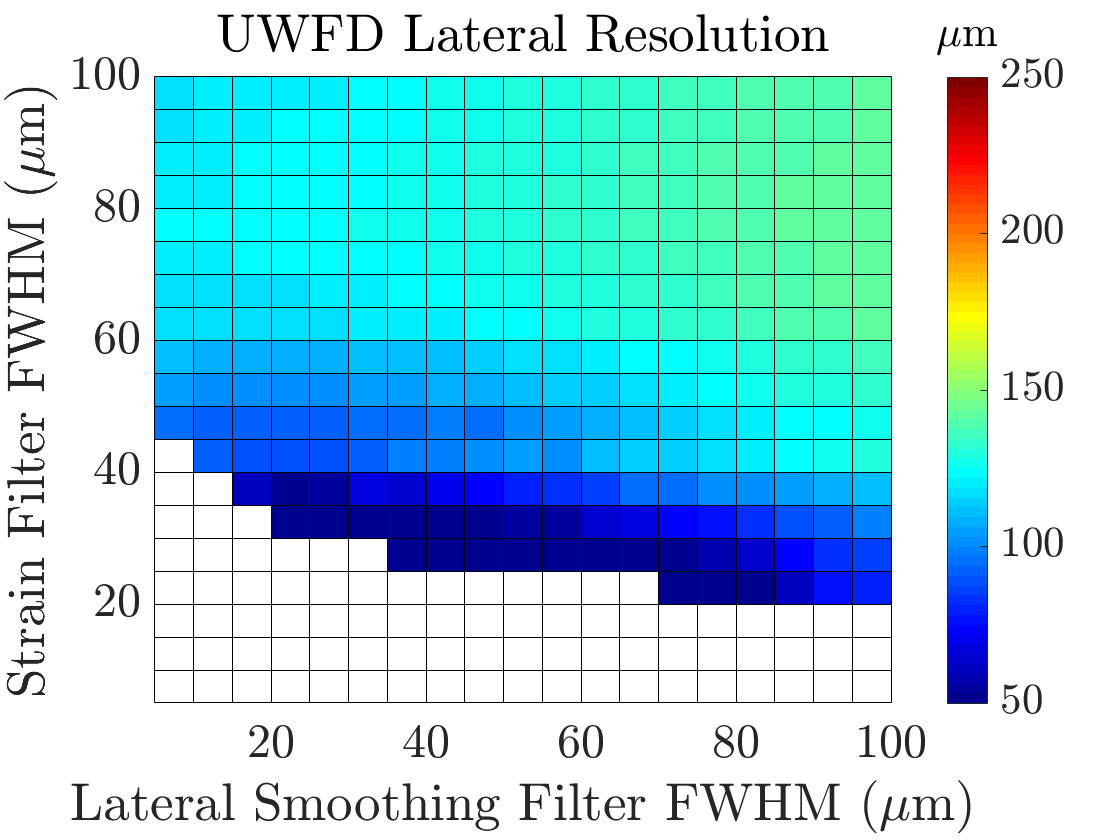
\includegraphics[width=\textwidth]{imageres_figs/uwfd_lateral.png}
	\end{subfigure}
	\\
	\begin{subfigure}{0.49\textwidth}
		\centering
		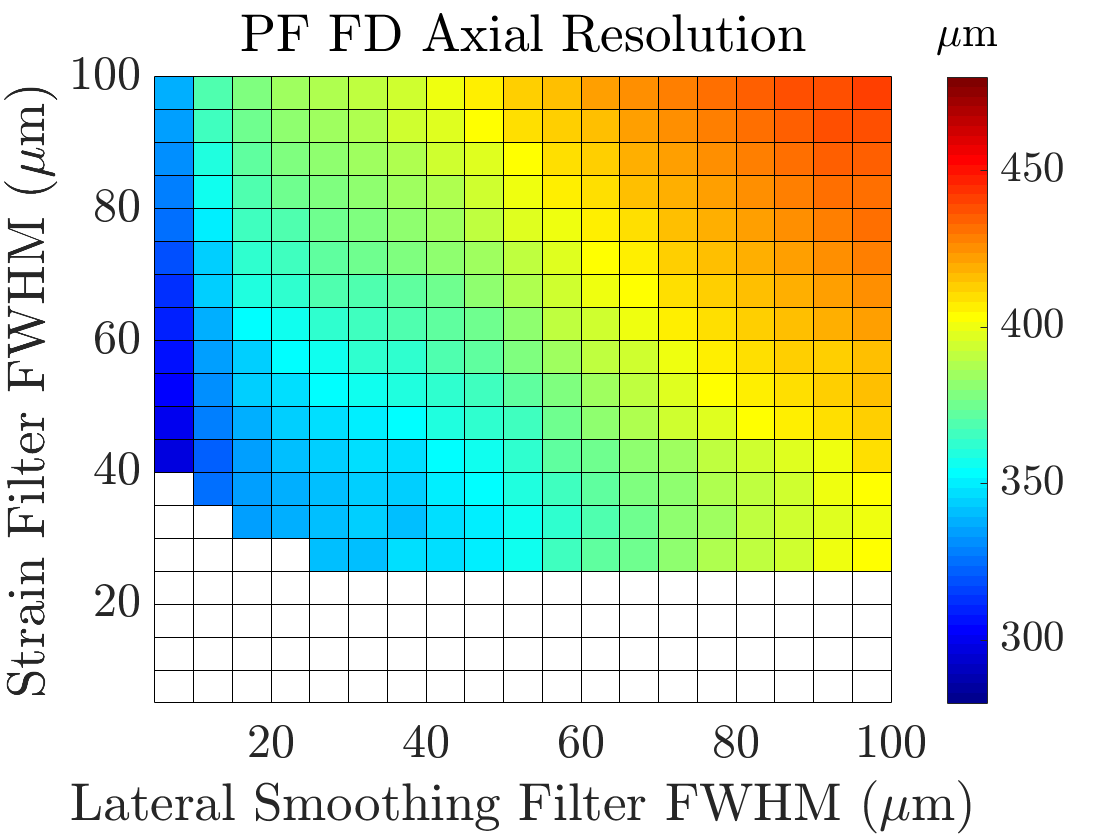
\includegraphics[width=\textwidth]{imageres_figs/pffd_axial.png}
	\end{subfigure}
	\begin{subfigure}{0.49\textwidth}
		\centering
		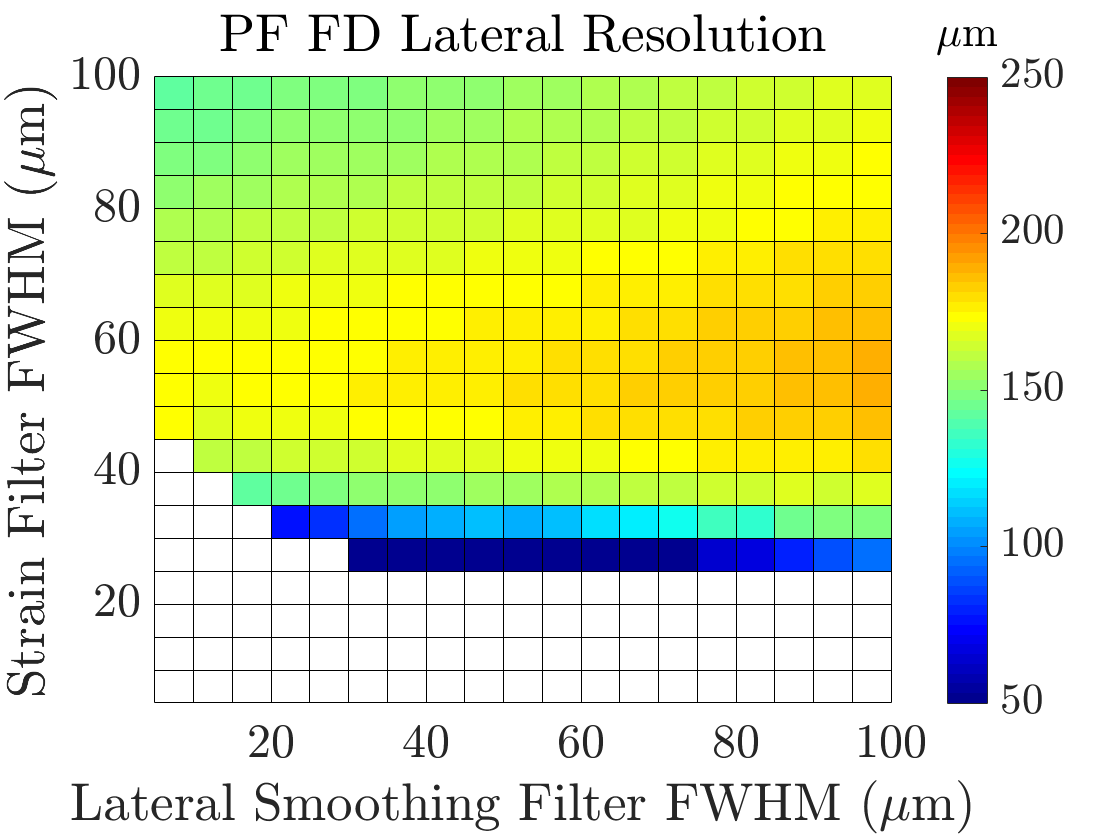
\includegraphics[width=\textwidth]{imageres_figs/pffd_lateral.png}
	\end{subfigure}
	\caption{The images on the left show the axial image resolution, and those on the right the lateral image resolution for the six different strain estimation techniques, at different strain and lateral smoothing filter FWHM resolutions.}
	\label{imageres_figs}
\end{figure}

Looking at these tables, it can be seen that the finite difference methods returned consistently lower axial image resolutions than the unwrapping with WLS and the offset phase with SG filtering, and was approximately equal to the unwrapping with SG filtering. The weighted FD method showed slightly better axial image resolution than the unweighted, whilst the pre-filtered FD with smoothing was larger than both. Overall, the unweighted smoothing with FD strain estimation showed the best axial image resolution. 
For the lateral image resolution, however, the unwrapping with WLS was much closer to the unweighted finite difference, and there was a less clear difference between the FD methods and the others. The weighted FD performed poorly, and the pre-filtered FD slightly better. 

Considering the results from the sections above, for both sensitivity and processing time, a closer look into the image resolution of the unweighted smoothing with FD was performed. In order to minimise the image resolutions (corresponding to maximising the ability to distinguish between fine structures in the sample) whilst also optimising the sensitivity, \autoref{uwfd_imageres} also shows the sensitivity for different fit lengths. Both plots show large image resolution values at high lateral smoothing and fit resolutions. In particular, an increased lateral smoothing leads to significant increase in the FWHM value for both axial and image resolutions. 

In summary, \autoref{wls_uwfd_compare} shows the previously used strain estimation technique at a standard fit resolution of $70\mu m$ and with no lateral smoothing, compared to the newly investigate unweighted smoothing with FD, with fit and lateral resolution parameters optimised ($\text{FR}=60\mu m$, $\text{LR}= 20\mu m$). The unweighted smoothing FD algorithm is  

\begin{figure}
	\centering
	\begin{subfigure}{0.49\textwidth}
		\centering
		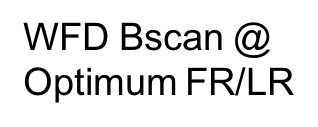
\includegraphics[width=\textwidth]{figures/uwfd_compare.png}
	\end{subfigure}
	\begin{subfigure}{0.49\textwidth}
		\centering
		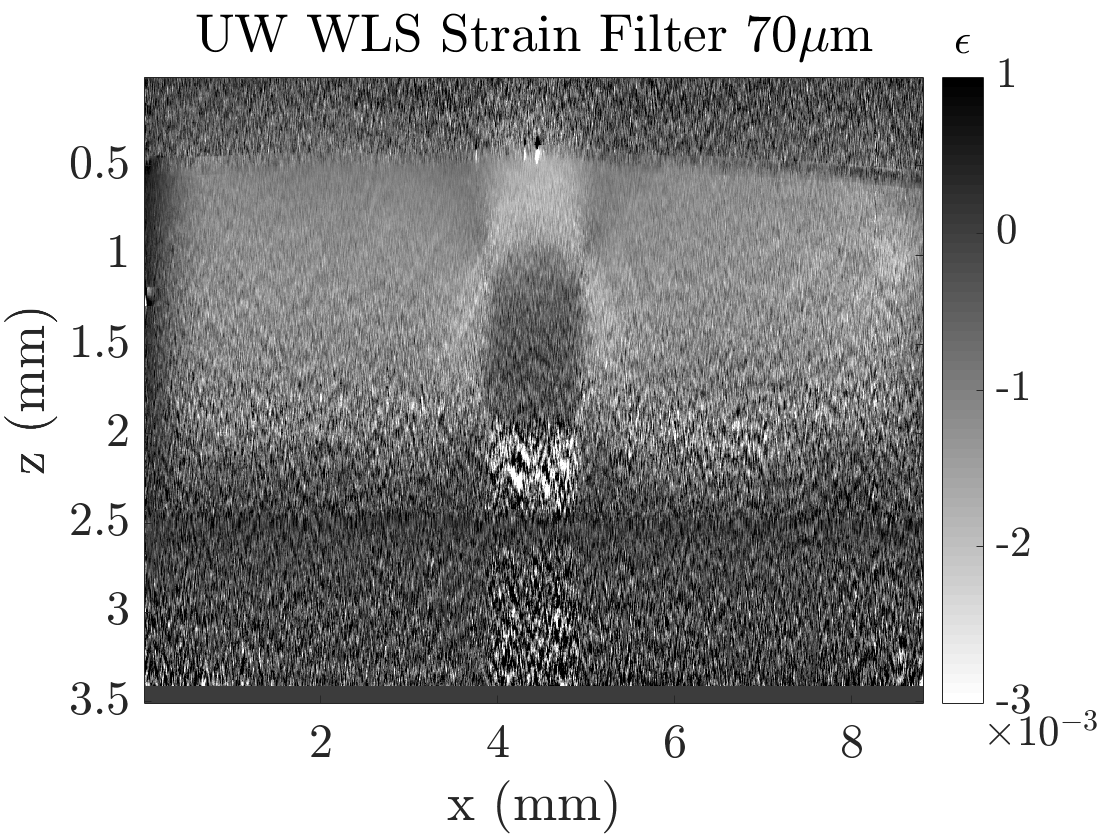
\includegraphics[width=\textwidth]{figures/wls_compare.png}
	\end{subfigure}
	\caption{Unweighted smoothing with FD strain estimation B-scan compared with the previously standard unwrapping with WLS.}
	\label{wls_uwfd_compare}
\end{figure}

